\chapter{Experiments} \label{chap-5}

This chapter presents the results of initial experimental studies of elliptical painting at the SNS. The simulations in chapter \ref{chap-2}-\ref{chap-3} were used to guide the experiments, and the diagnostics described in chapter \ref{chap-4} were used to measure the painted distribution. Recall from chapter \ref{chap-3} that solenoid magnetic fields should help the distribution remain close to a Danilov distribution during injection; solenoid magnets were planned to be installed in the SNS ring in 2021, but their installation was delayed until mid-2022, outside the timeframe of this dissertation. Thus, the beams created in the following experiments were not expected to be optimal. Nonetheless, it was hoped that the beams would be clearly distinguishable from a production beam produced by correlated painting. 


\section{Procedure}

Accelerator physics experiments are performed in the SNS control room using the OpenXAL framework. OpenXAL provides a high-level interface to perform tasks such as changing magnet strengths, triggering the beam, etc. It can also perform single-particle or envelope tracking using an online model of the accelerator. OpenXAL scripts are written in Java or Jython and are executed from the command line. Many graphical user interface (GUI) OpenXAL applications have been developed over the history of the SNS and are available for use in the control room. 

The following steps are taken during the experimental setup:
%
\begin{enumerate}
    \item 
    The beam energy is lowered from 1.0 GeV to 0.8 GeV by turning off several RF cavities at the end of the linac. This is performed by the SNS operations team. Generally, lowering the energy causes other accelerator components to trip or malfunction due to the modified timing system; these must be corrected one-by-one. The first attempt to lower the energy to 0.8 GeV took over six hours.
    %
    \item
    The horizontal and vertical tunes are set to the same value using the Ring Optics Control (ROC) application. ROC varies several quadrupoles until the model tunes are equal to the desired tunes. The tunes are measured using turn-by-turn BPM readings from a single minipulse in the ring. Generally, the measured and model tunes are not quite equal; we therefore shift the ROC input tunes until the measured tunes converge to the desired tunes. 
    %
    \item
    (Optional: Modify the injection region in some way to assist the injection kickers.)
    %
    \item
    The eight injection kicker magnets are calibrated using the Ring Injection Control (RIC) application, as described in chapter \ref{chap-1}. 
    %
    \item
    The initial/final kicker voltages are determined to obtain the desired closed-orbit coordinates at the foil, as described in chapter \ref{chap-1}.
    %
    \item
    The initial/final voltages are connected with a square root waveform; the waveform is applied to the injection kickers. The duration of the waveform — the painting time — is chosen at this step but can be easily changed later on. The painting time determines the number of minipulses in the final distribution; i.e., the beam intensity.
    %
    \item
    The number of injected turns before extraction is chosen. This allows the distribution to be measured at different times during injection.  It is also possible to store the beam in the ring, although the SNS normally extracts the beam immediately after accumulation.
    %
\end{enumerate}
%
The next task is to prepare for the measurements. For the wire-scanner measurement, the first step is to modify the RTBT optics using the application developed as part of this dissertation. If the fixed-optics method is used, the optics are changed immediately. If the multi-optics method is used, the optics are pre-computed and stored for later use. The SNS employs a sophisticated machine protection system (MPS) that will cause the machine to trip if the RTBT quadrupole strengths wander outside a certain window, so this window is extended beforehand. Additionally, MPS will activate if the fractional change in field strength is too large; to solve this problem, the field strength is changed in small steps. Wire-scanner data acquisition is performed by the Profile Tools and Analysis (PTA) application. The beam is set to a pulse frequency of 1 Hz, and the beam loss monitors in the wire-scanner region are masked due to the higher-than-normal losses when the wires cross the beam core. After the four wire-scanners complete their scan, a time-stamped file is produced containing the measured profiles.

The second measurement is the tomographic reconstruction from $x$-$y$ projections on the target. Since the optics calculation is time-consuming, it can be run in the background while wire-scans are collected. The target images for tomographic reconstruction was proposed late in this research, so the target scan was only performed in the last of the following experiments.


\section{Experiment 1}

The SNS reserves approximately one day per month for accelerator physics experiments, and various experiments must compete for time within this twenty-four hour period. At the time of our first experiment, setup of the injection region using the RIC application had not yet been completed. Although simulations indicated that the kickers were not strong enough to perform elliptical painting at 1 GeV kinetic energy, this had not been tested. And the SNS energy had not yet been decreased — a time-consuming and possibly error-prone task. The goal of Experiment 1 was therefore to push the injected coordinates $x$ and $y'$ to their limits at 1 GeV.

Simulations predict that the distribution will undergo significant change during injection, especially without the presence of solenoid magnets in the ring; therefore, it is interesting to measure the distribution not only at its final state, but also at the intermediate states. Using the fixed-optics method, ten measurements can be performed within one hour. 

\subsection{Experiment 1a: correlated painting}

Before setting up for elliptical painting, a production beam was measured for comparison. Recall that a production beam is produced using correlated painting: the displacements at the foil are increased from an initial offset to their final value, and the slope at the foil is always zero. The number of injected turns was reduced from 1000 to 500, and the beam was measured every 50 turns. 

The measured wire-scanner profiles are shown in Fig.~\ref{fig:exp1a_wsmeas}, and the reconstructed emittances and covariance ellipses at BPM17, just before QH18, are shown in Fig.~\ref{fig:exp1a_emittances}.
%
\begin{figure}[!p]
    \centering
    \begin{subfigure}{\textwidth}
        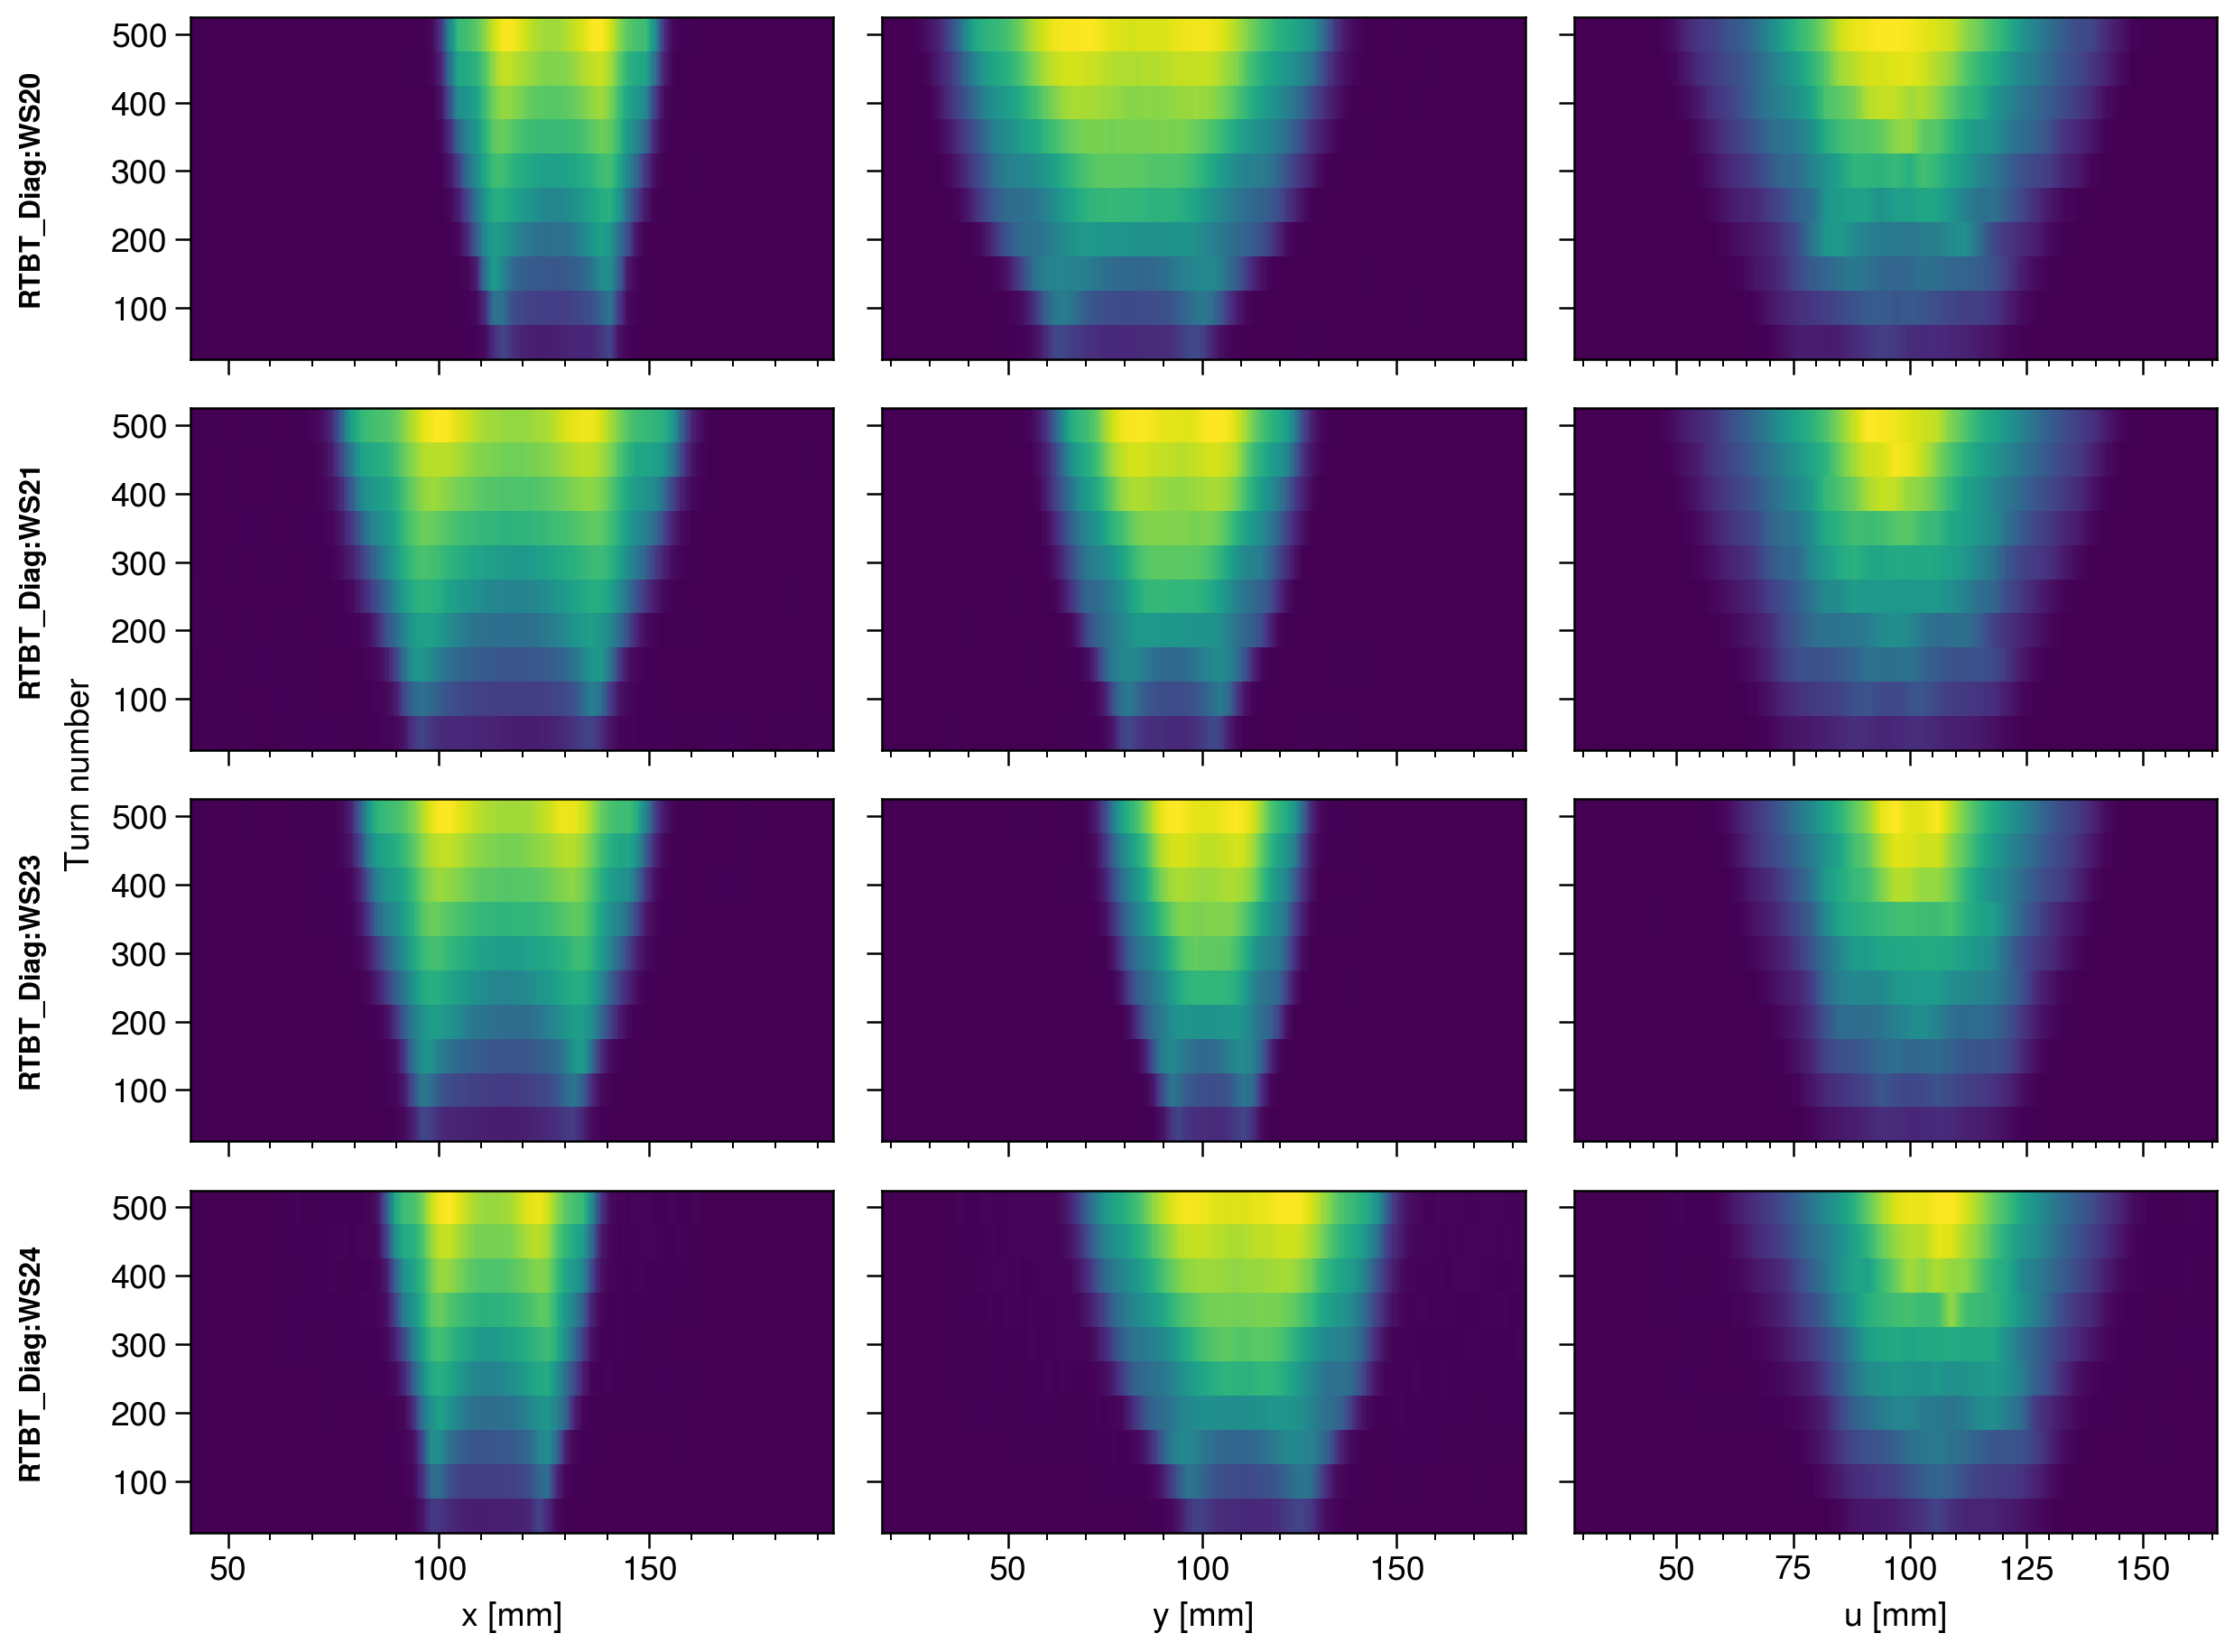
\includegraphics[width=\textwidth]{Images/chapter5/exp1a/waterfall.png}
    \end{subfigure}
    \vfill
    \vspace*{1.25cm}
    \vfill
    \begin{subfigure}{\textwidth}
        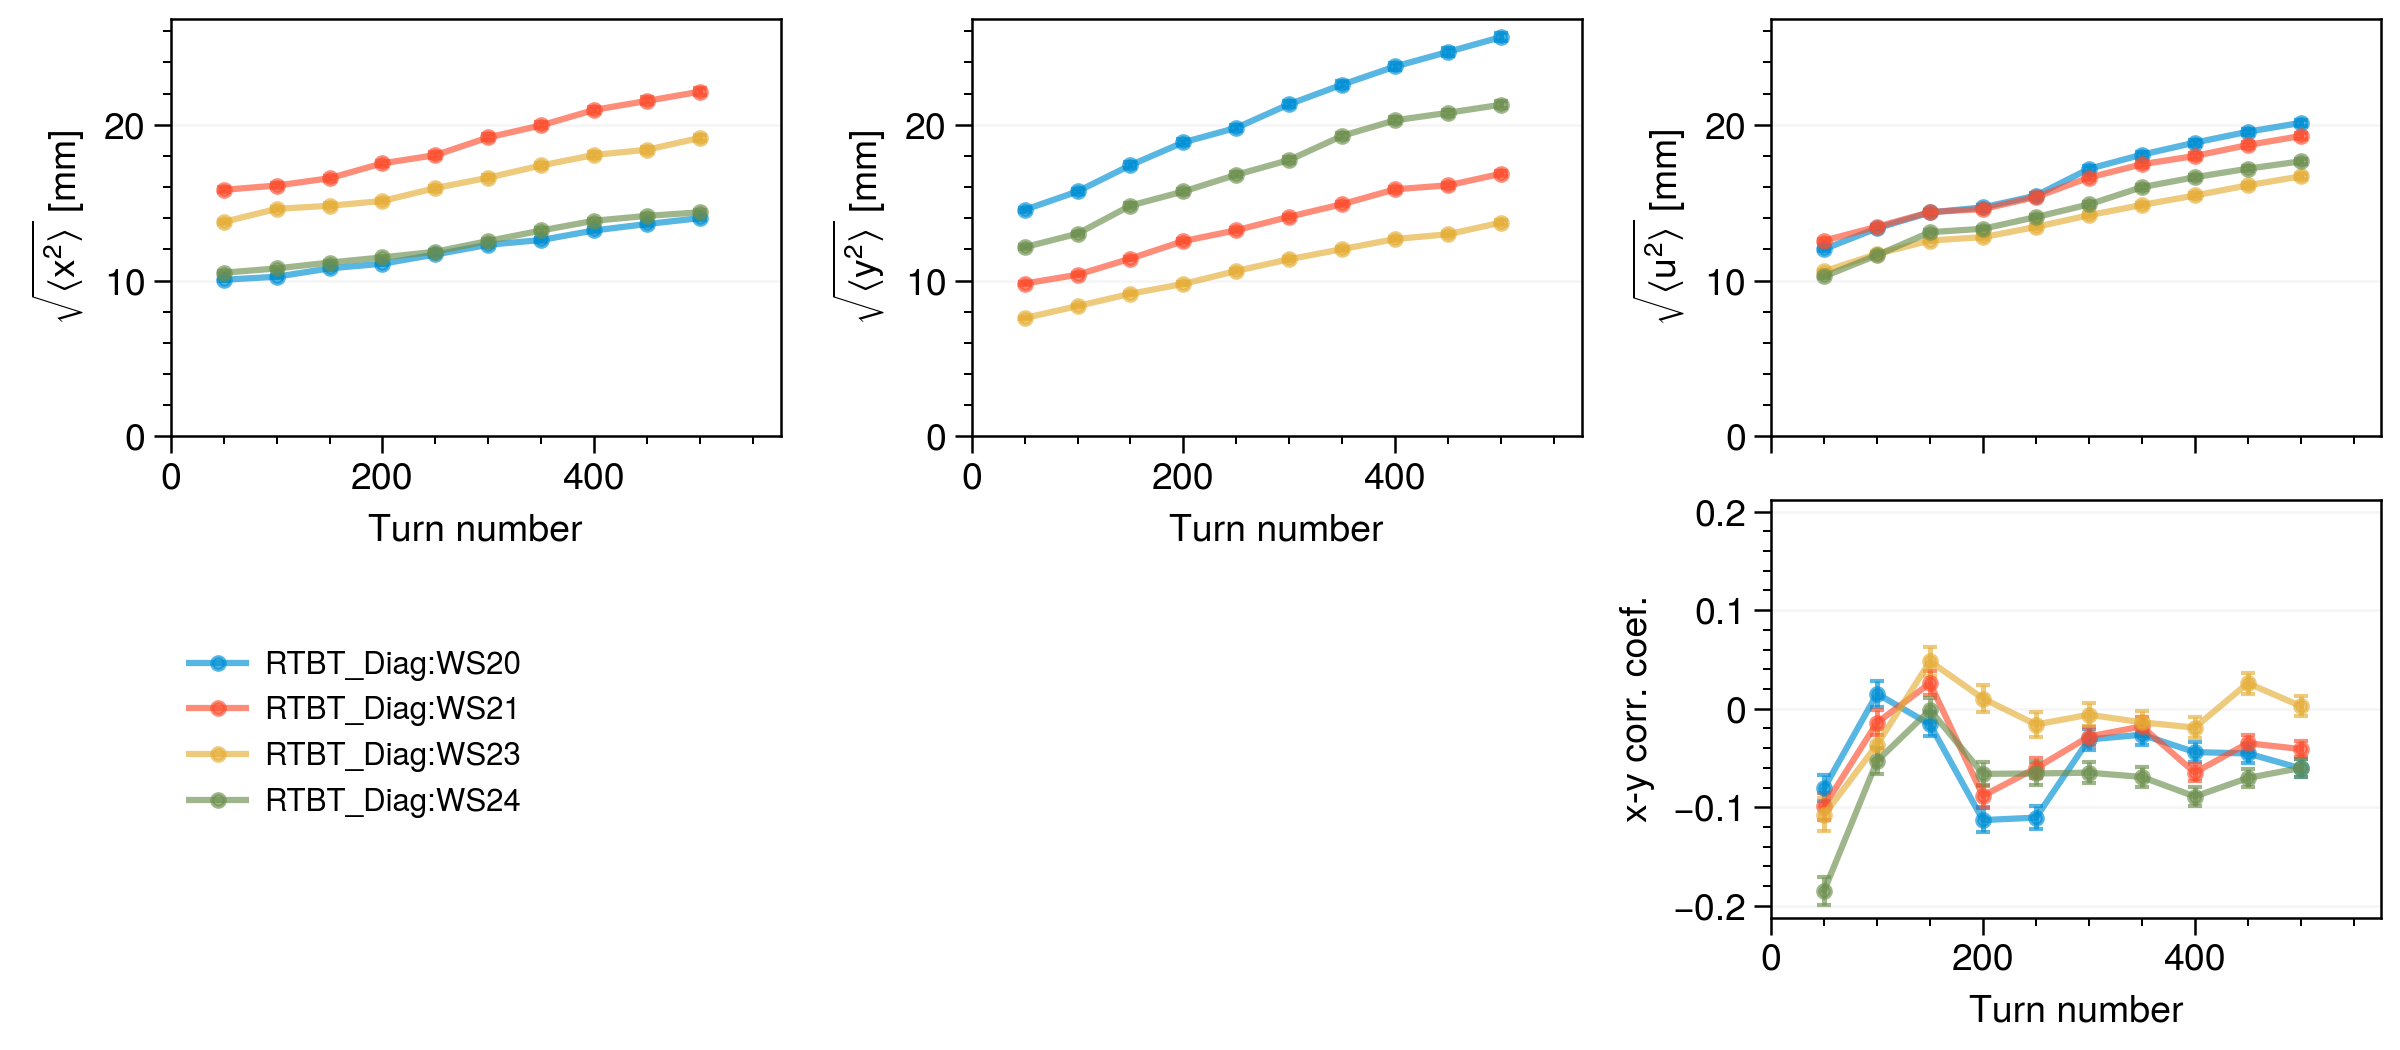
\includegraphics[width=\textwidth]{Images/chapter5/exp1a/rms.png}
    \end{subfigure}
    \caption{Measured wire-scanner profiles from Experiment 1a.}
    \label{fig:exp1a_wsmeas}
\end{figure}
%
%
\begin{figure}[!p]
    \centering
    \begin{subfigure}{0.6\textwidth}
        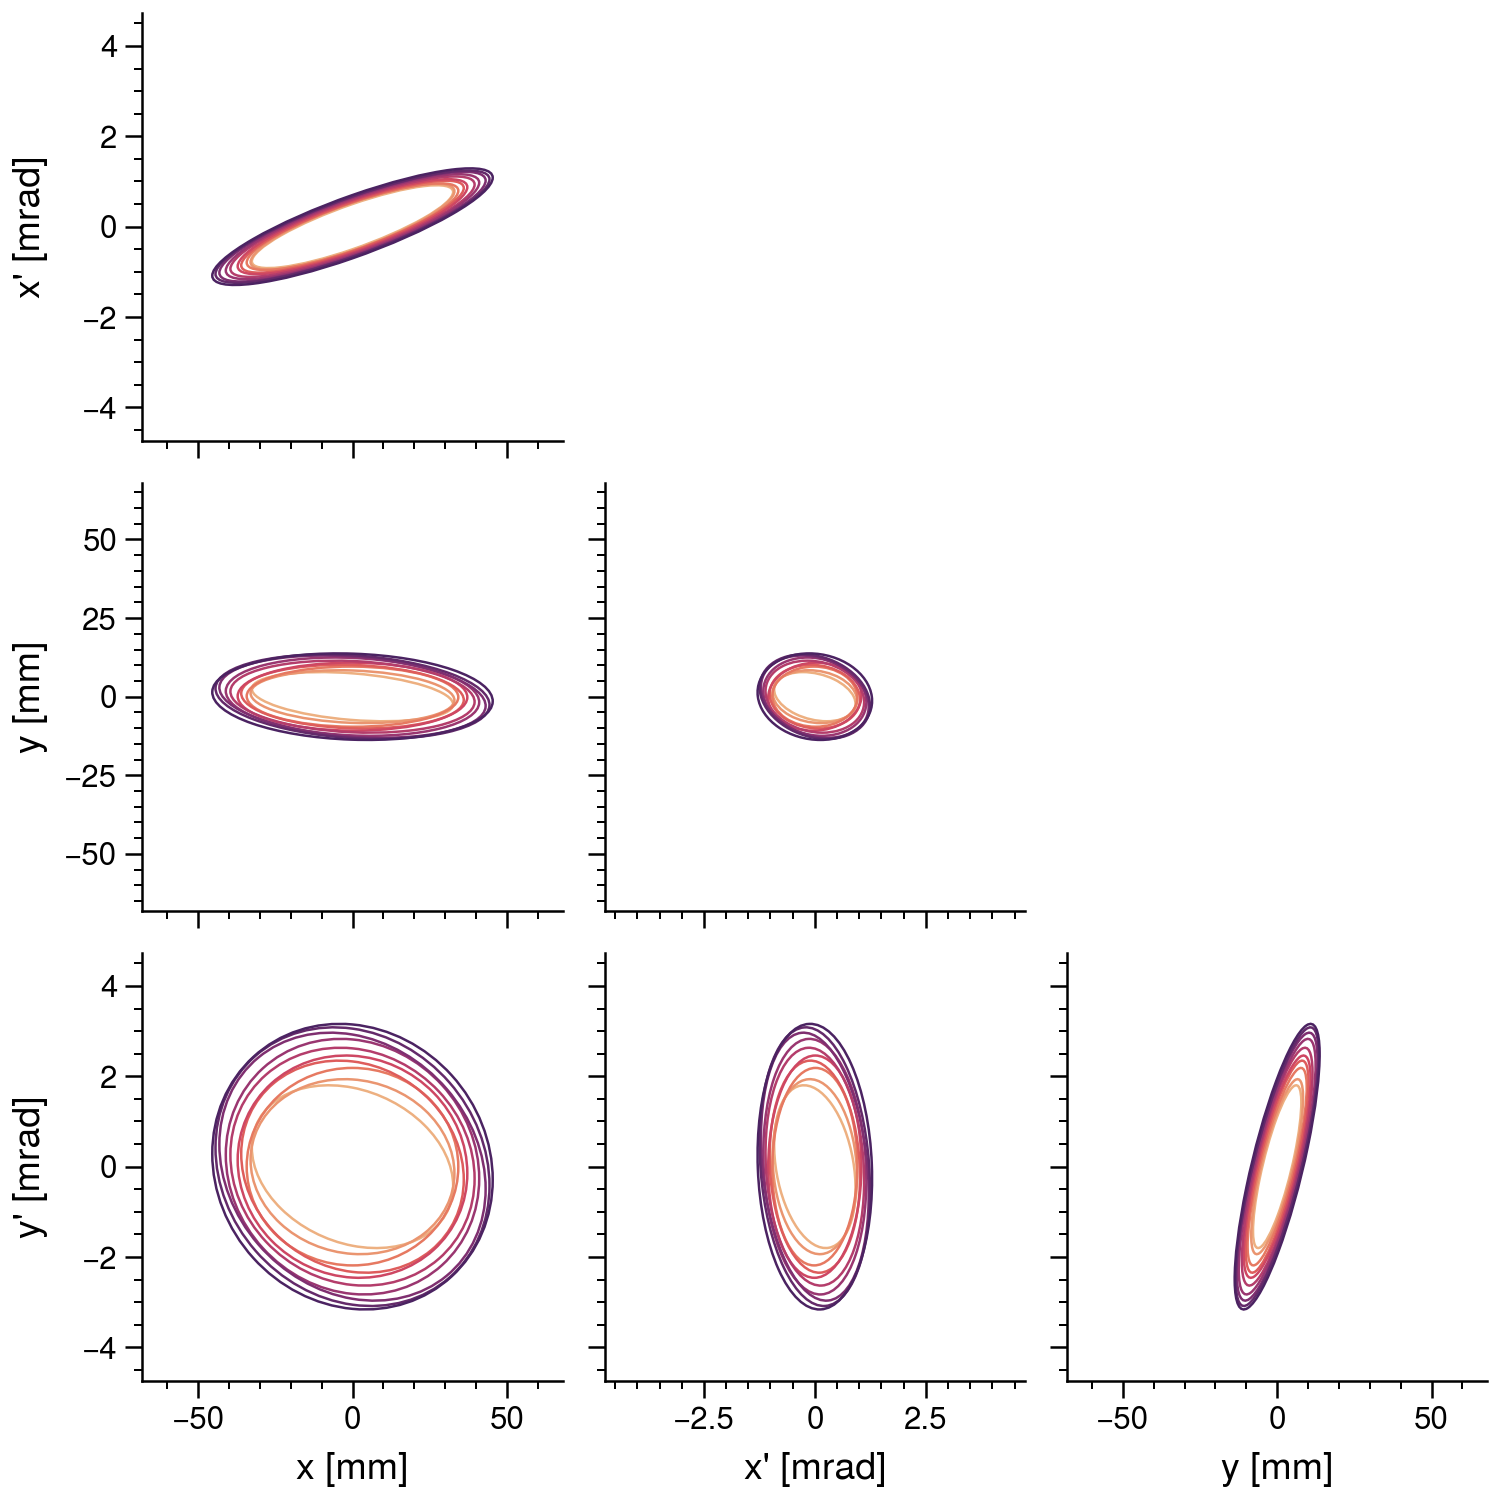
\includegraphics[width=\textwidth]{Images/chapter5/exp1a/corner.png}
    \end{subfigure}
    \hfill
    \begin{subfigure}[t]{0.39\textwidth}
        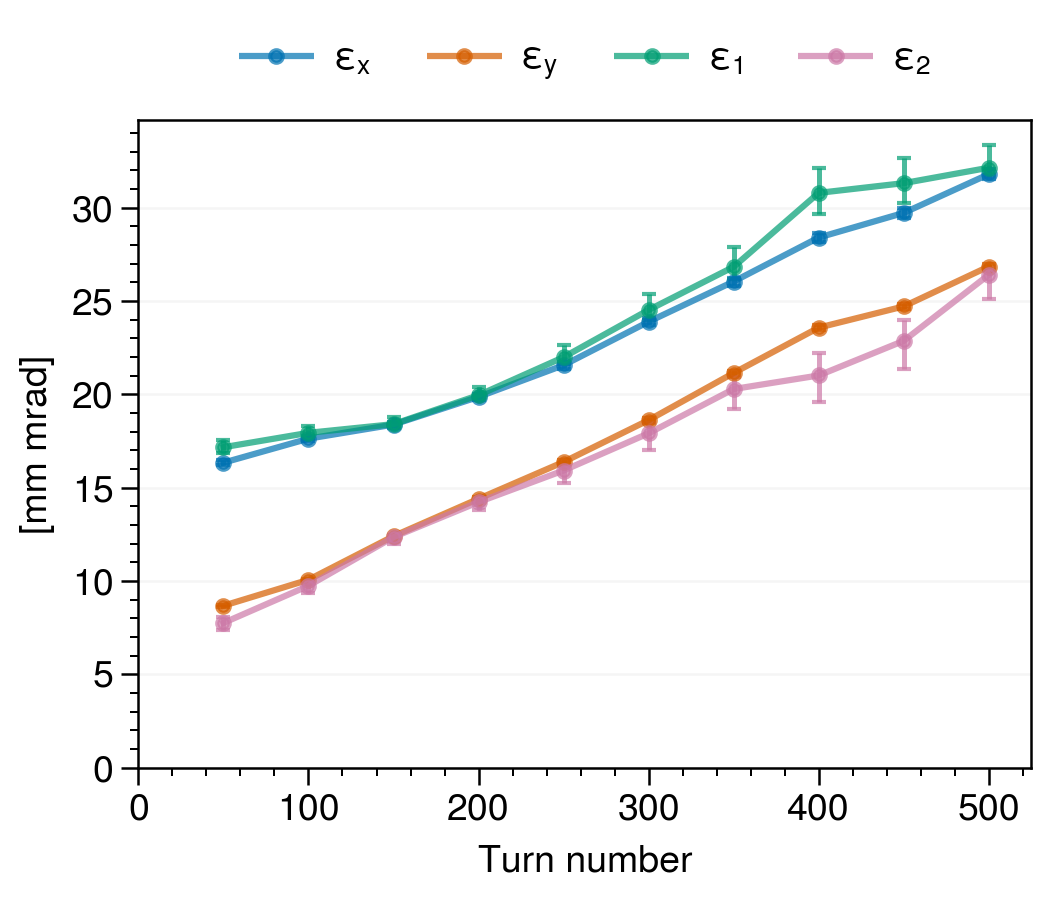
\includegraphics[width=\textwidth]{Images/chapter5/exp1a/emittances.png}
    \end{subfigure}
    \caption{Reconstructed emittances and covariance ellipses from Experiment 1a. In this and subsequent figures, the reconstruction is performed at BPM17 and the light/dark ellipses correspond to the start/end of injection.}
    \label{fig:exp1a_emittances}
\end{figure}
%
Each subplot in Fig.~\ref{fig:exp1a_wsmeas} shows the evolution of the projection onto a single wire during injection; each row corresponds to a different wire-scanner and each column corresponds to a different projection axis — $x$, $y$, or $u$. That the closed orbit starts offset from the foil is evident from initial two peaks in the $x$ and $y$ projections. The distribution forms a ring or donut in $x$-$x'$ and $y$-$y'$, and the hollow center eventually becomes partially filled due to space charge and other nonlinear effects.

The main feature of Fig.~\ref{fig:exp1a_emittances} is that there is very little measured cross-plane correlation in the beam, as expected for the correlated painting method. The error bars are calculated by repeating the reconstruction many times with noise added to the measured moments, then taking the mean and standard deviation over the trials. This can lead to asymmetric error bars, which will be shown in the next sections. (Previous measurements indicate that the moments estimated from the profiles have less than 2\% variation if repeated multiple times.)

It is also possible to reconstruct the covariance matrix at different locations in the lattice. Fig.~\ref{fig:exp1a_rec_betas_throughout} shows the reconstructed $\beta$ functions throughout the RTBT.
%
\begin{figure}[!p]
    \centering
    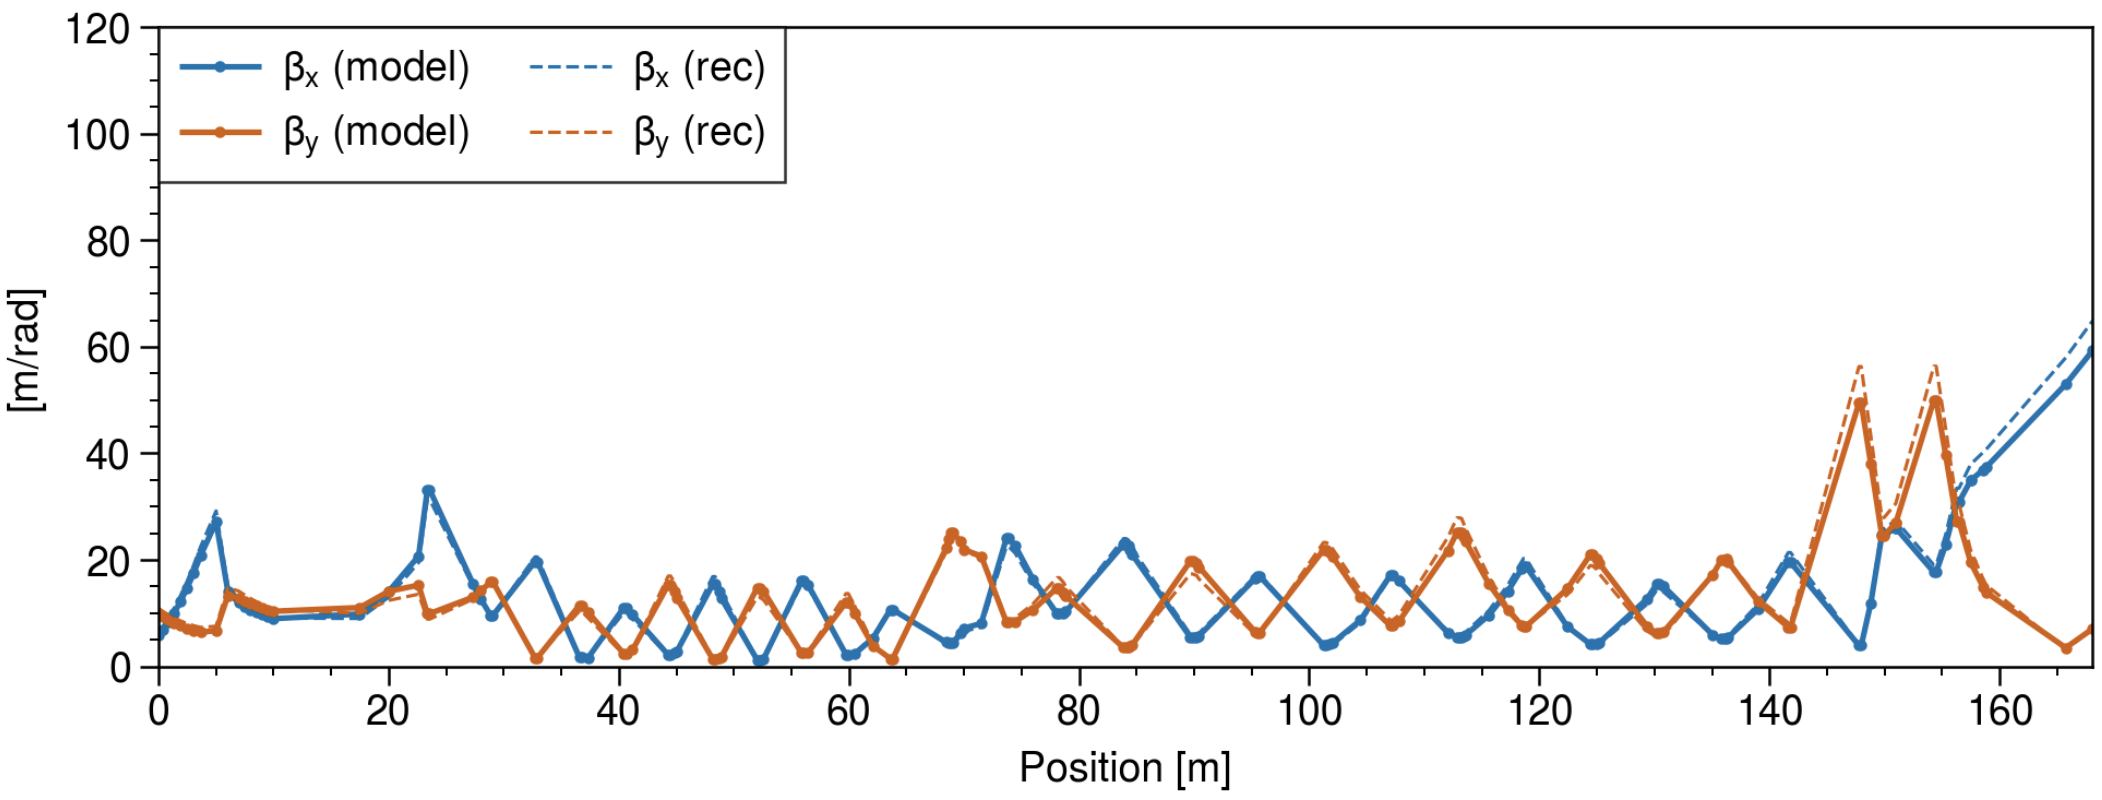
\includegraphics[width=1.0\textwidth]{Images/chapter5/exp1a/rec_betas_throughout.png}
    \caption{Reconstructed $\beta$ functions from Experiment 1a.}
    \label{fig:exp1a_rec_betas_throughout}
\end{figure}
%
The model parameters are computed from the linear transfer matrix of the ring + RTBT. 


[Simulation]





\subsection{Experiment 1b: elliptical-ish painting}

Next, we attempted to carry out elliptical painting. First, [as shown in Fig.~\ref{},] the horizontal and vertical tunes were set to 6.18. The next step was to move the closed orbit to the foil. This was found to be possible in the vertical plane but impossible in the horizontal plane; the minimum distance from the foil was 10 mm. Additionally, the maximum possible vertical slope was 0.7 mrad. It was decided to continue with the painting method using initial coordinates: ($x$, $x'$, $y$, $y'$) $\approx$ (10 mm, 0 mrad, 0 mm, 0 mrad) and final coordinates: ($x$, $x'$, $y$, $y'$) $\approx$ (21 mm, 0 mrad, 0 mm, 0.7 mrad). The initial beam would be a donut in $x$-$x'$ and a point in $y$-$y'$. In real space, it would be a flat horizontal line with higher density on the two ends of the line. In other words, injected particles would move along an ellipse in the $x$-$y$ plane with zero vertical size. As time progressed, the horizontal and vertical size of the ellipse would grow at different rates depending on the maximum painting $x$ and $y'$ coordinates. This is all assuming linear transport and non-interacting particles. Without a computer, it is unclear what would happen with the inclusion of space charge.

[... We should probably show some screenshots of the RIC application. Maybe not here, but somewhere. ...]

The measured wire-scanner profiles are shown in Fig.~\ref{fig:exp1b_wsmeas}, and the reconstructed emittances and covariance ellipses at BPM17 are shown in Fig.~\ref{fig:exp1a_emittances}.
%
\begin{figure}[!p]
    \centering
    \begin{subfigure}{\textwidth}
        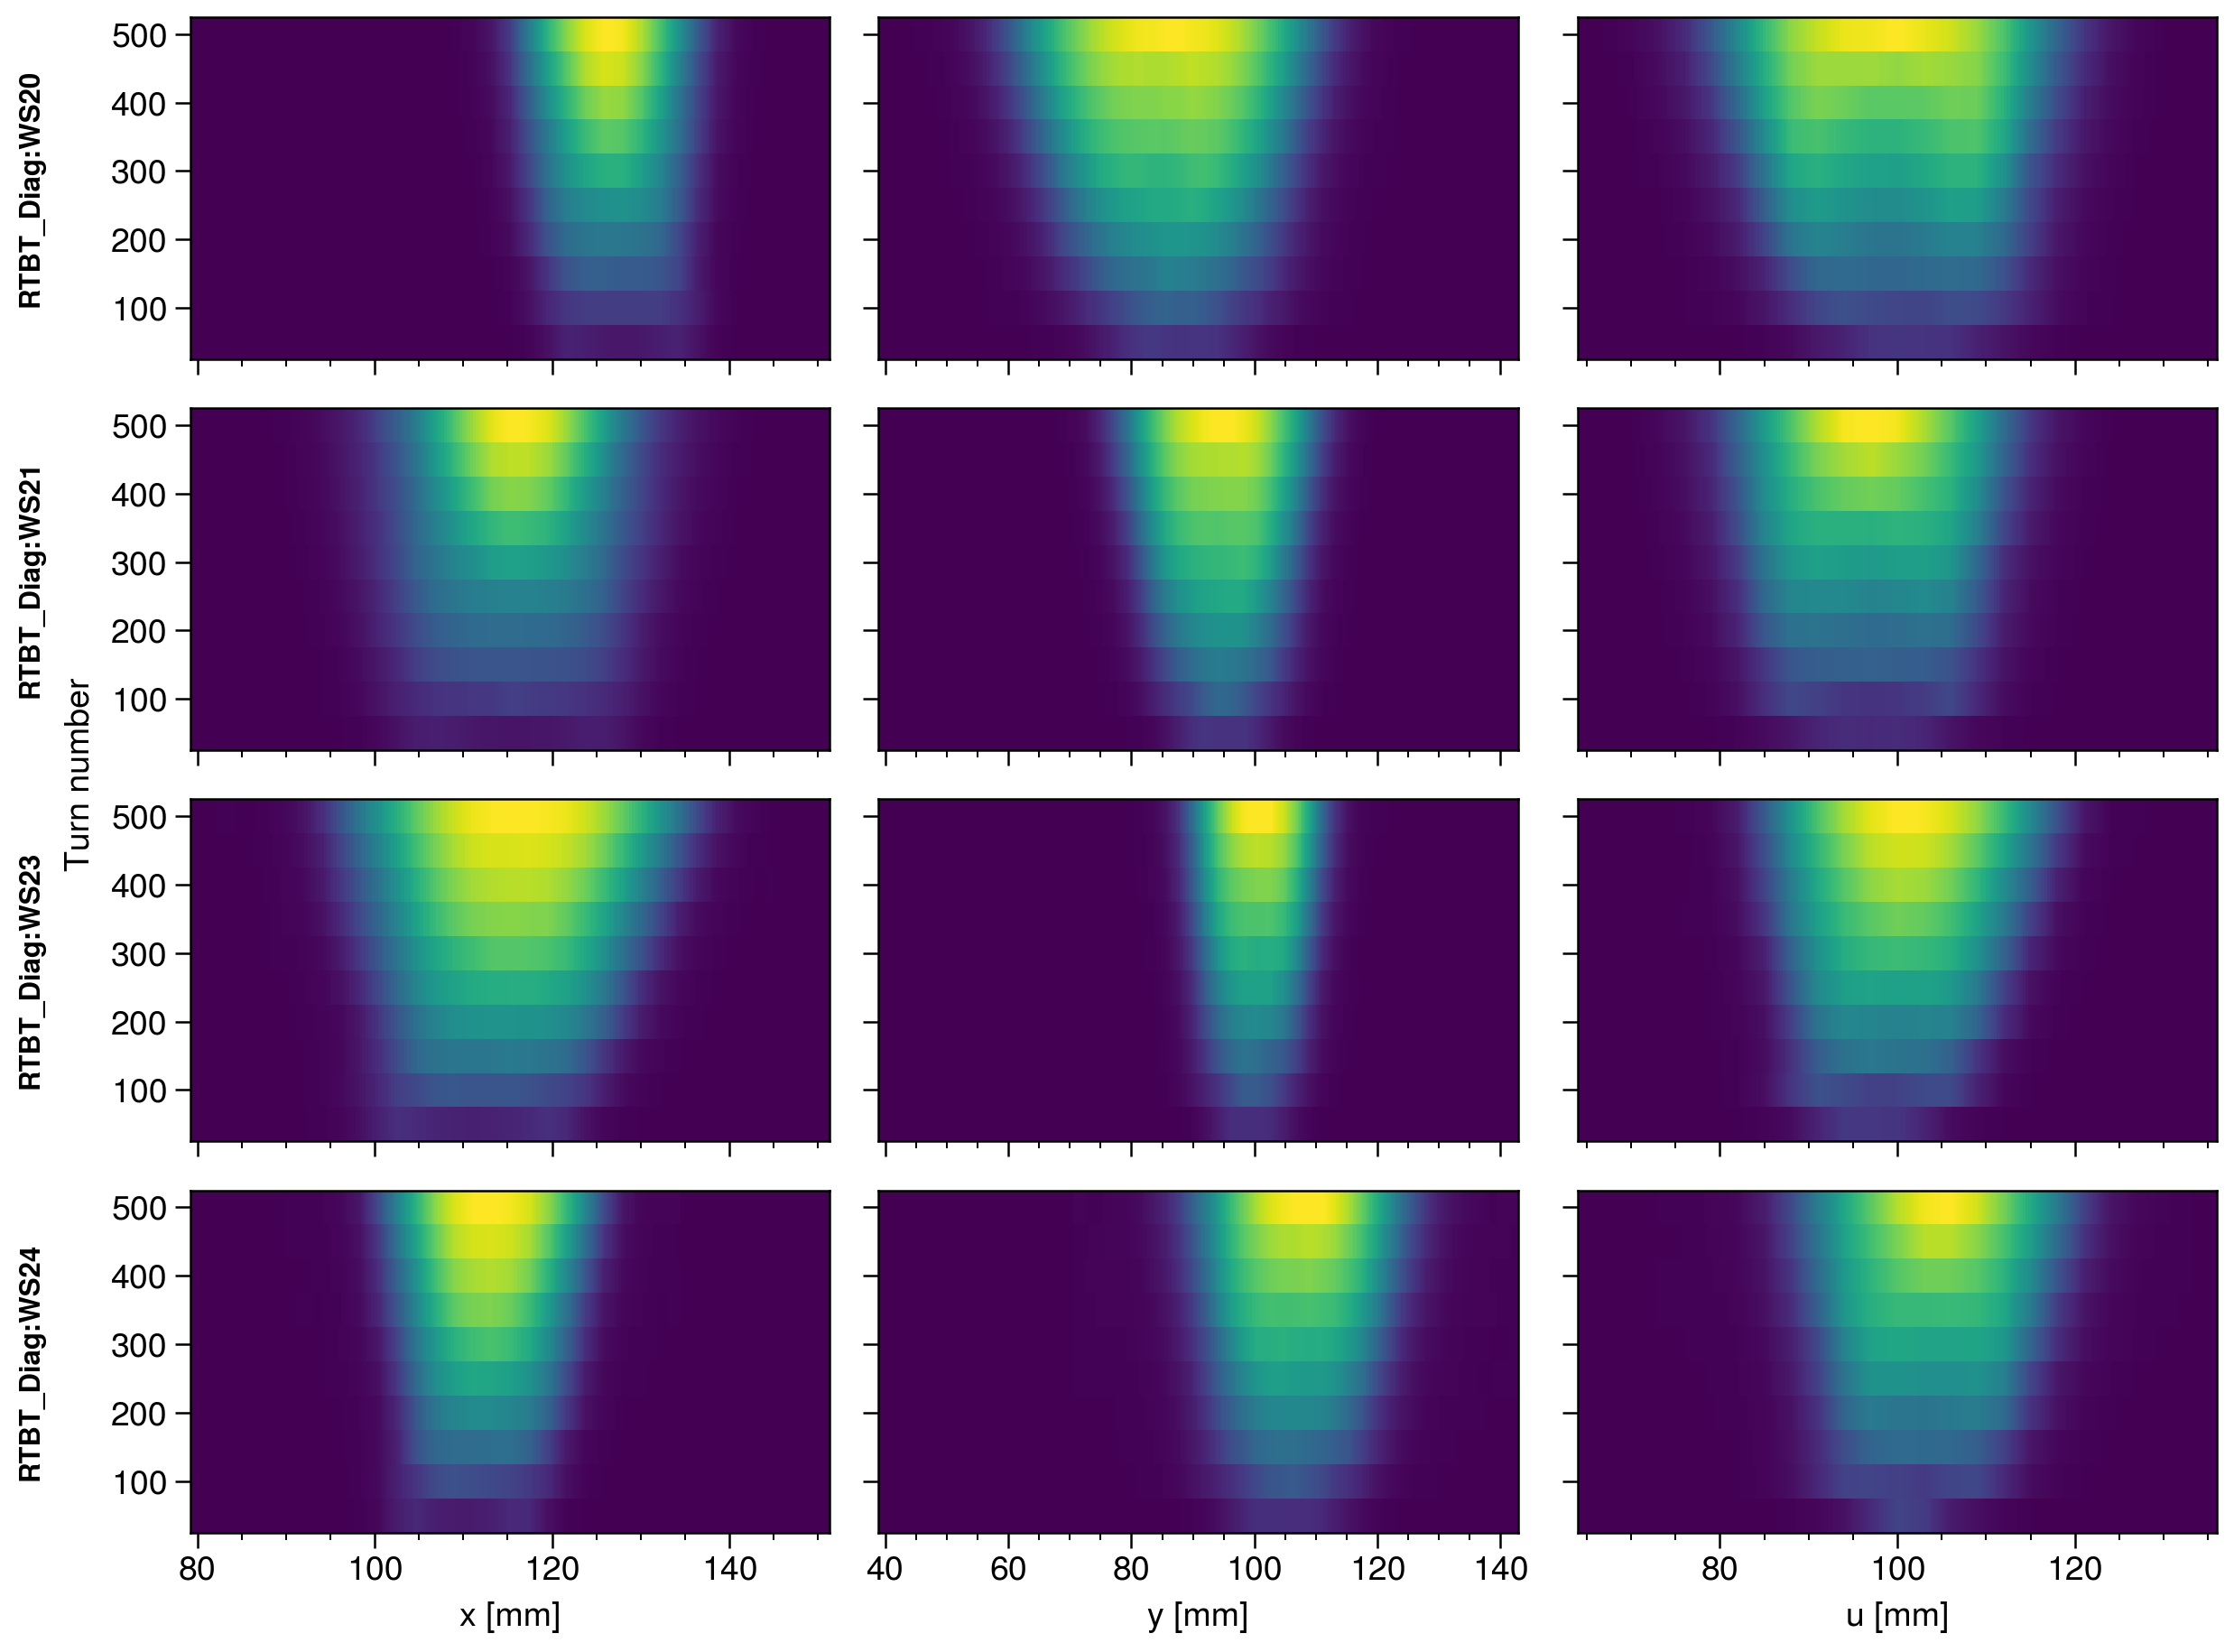
\includegraphics[width=\textwidth]{Images/chapter5/exp1b/waterfall.png}
    \end{subfigure}
    \vfill
    \vspace*{1.25cm}
    \vfill
    \begin{subfigure}{\textwidth}
        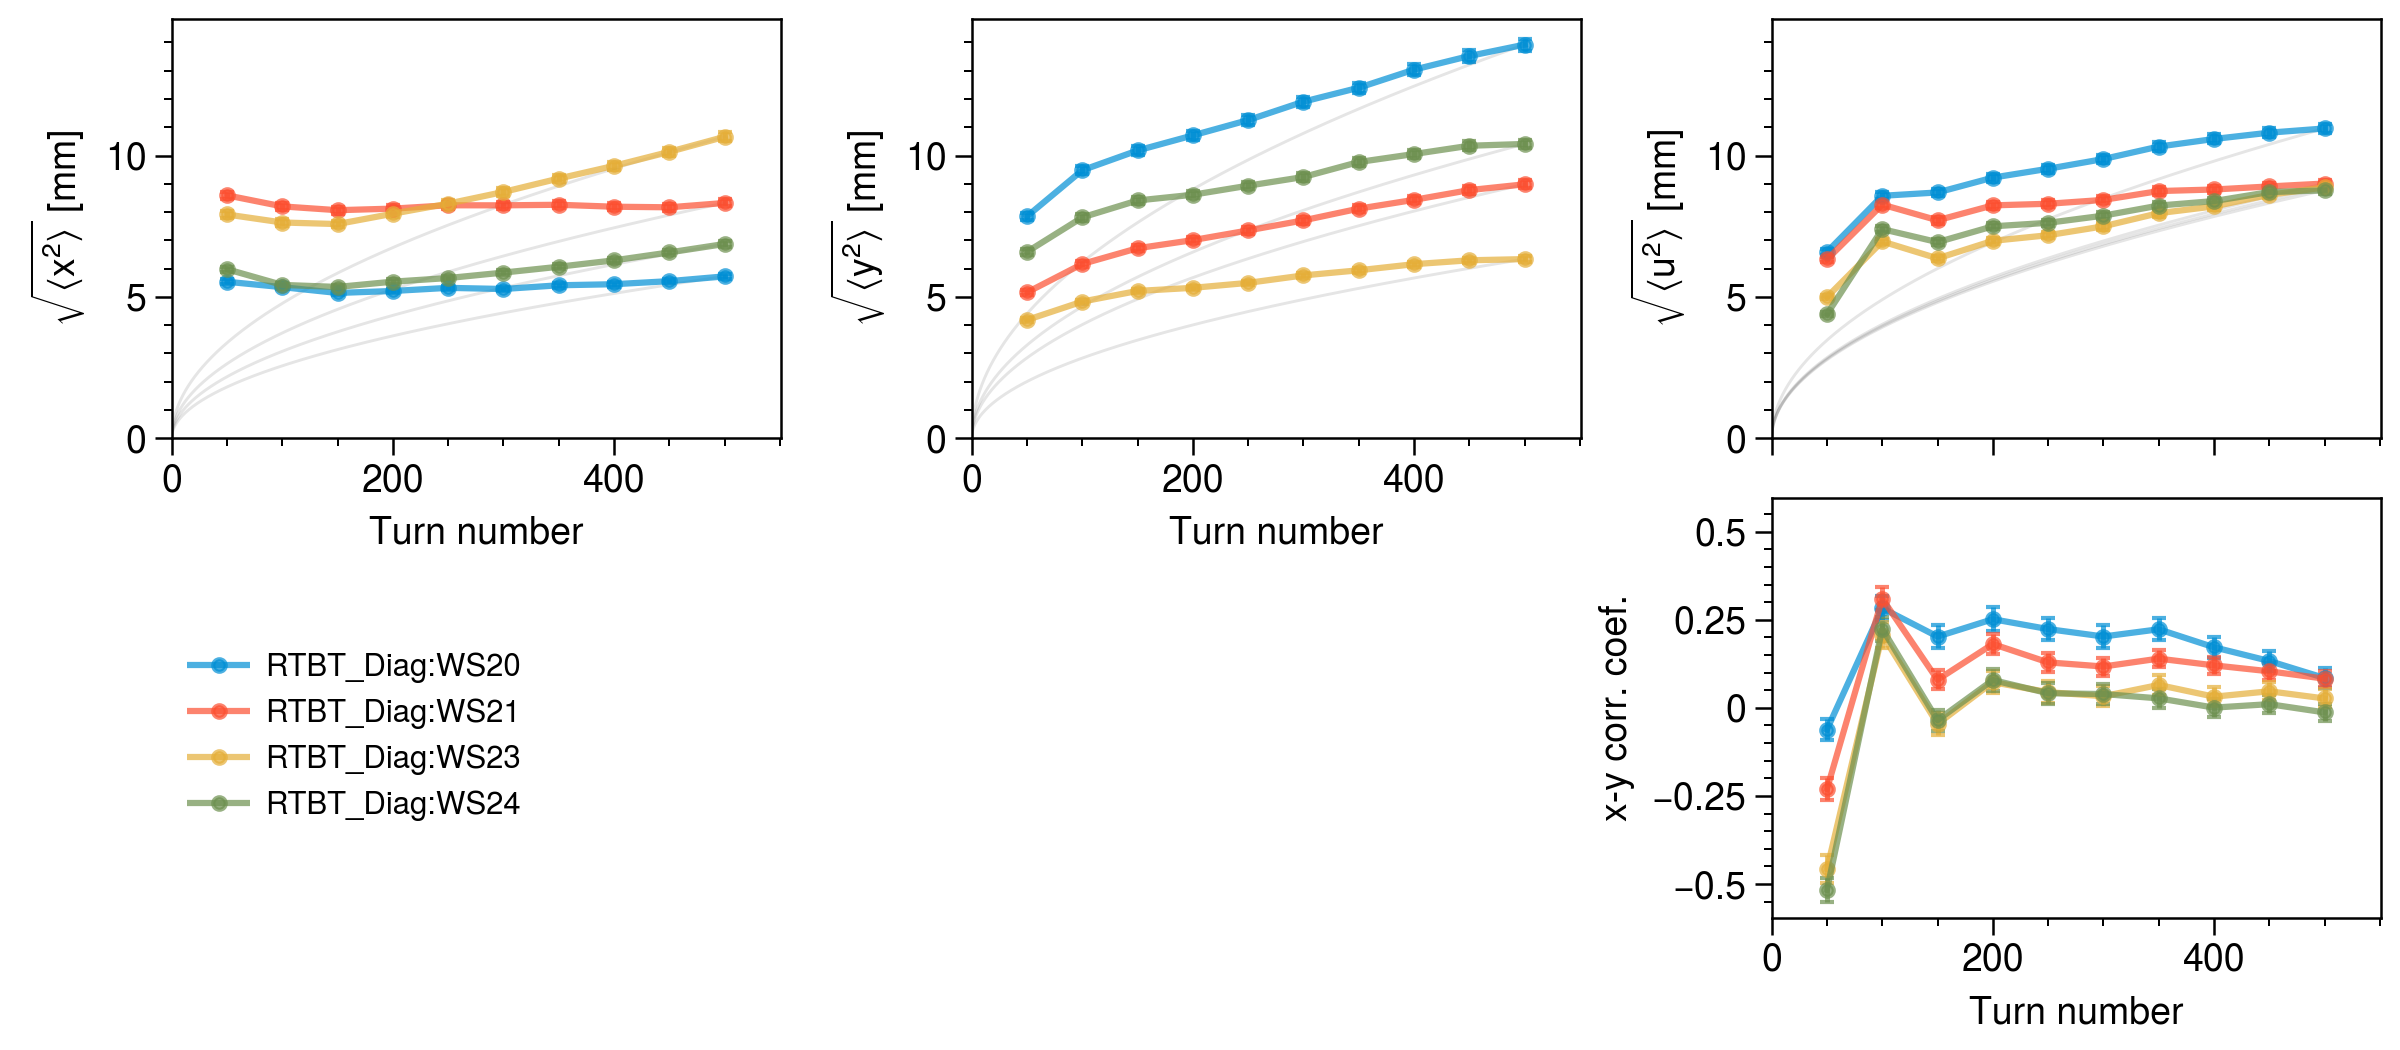
\includegraphics[width=\textwidth]{Images/chapter5/exp1b/rms.png}
    \end{subfigure}
    \caption{Measured wire-scanner profiles from Experiment 1b.}
    \label{fig:exp1b_wsmeas}
\end{figure}
%
%
\begin{figure}[!p]
    \centering
    \begin{subfigure}{0.6\textwidth}
        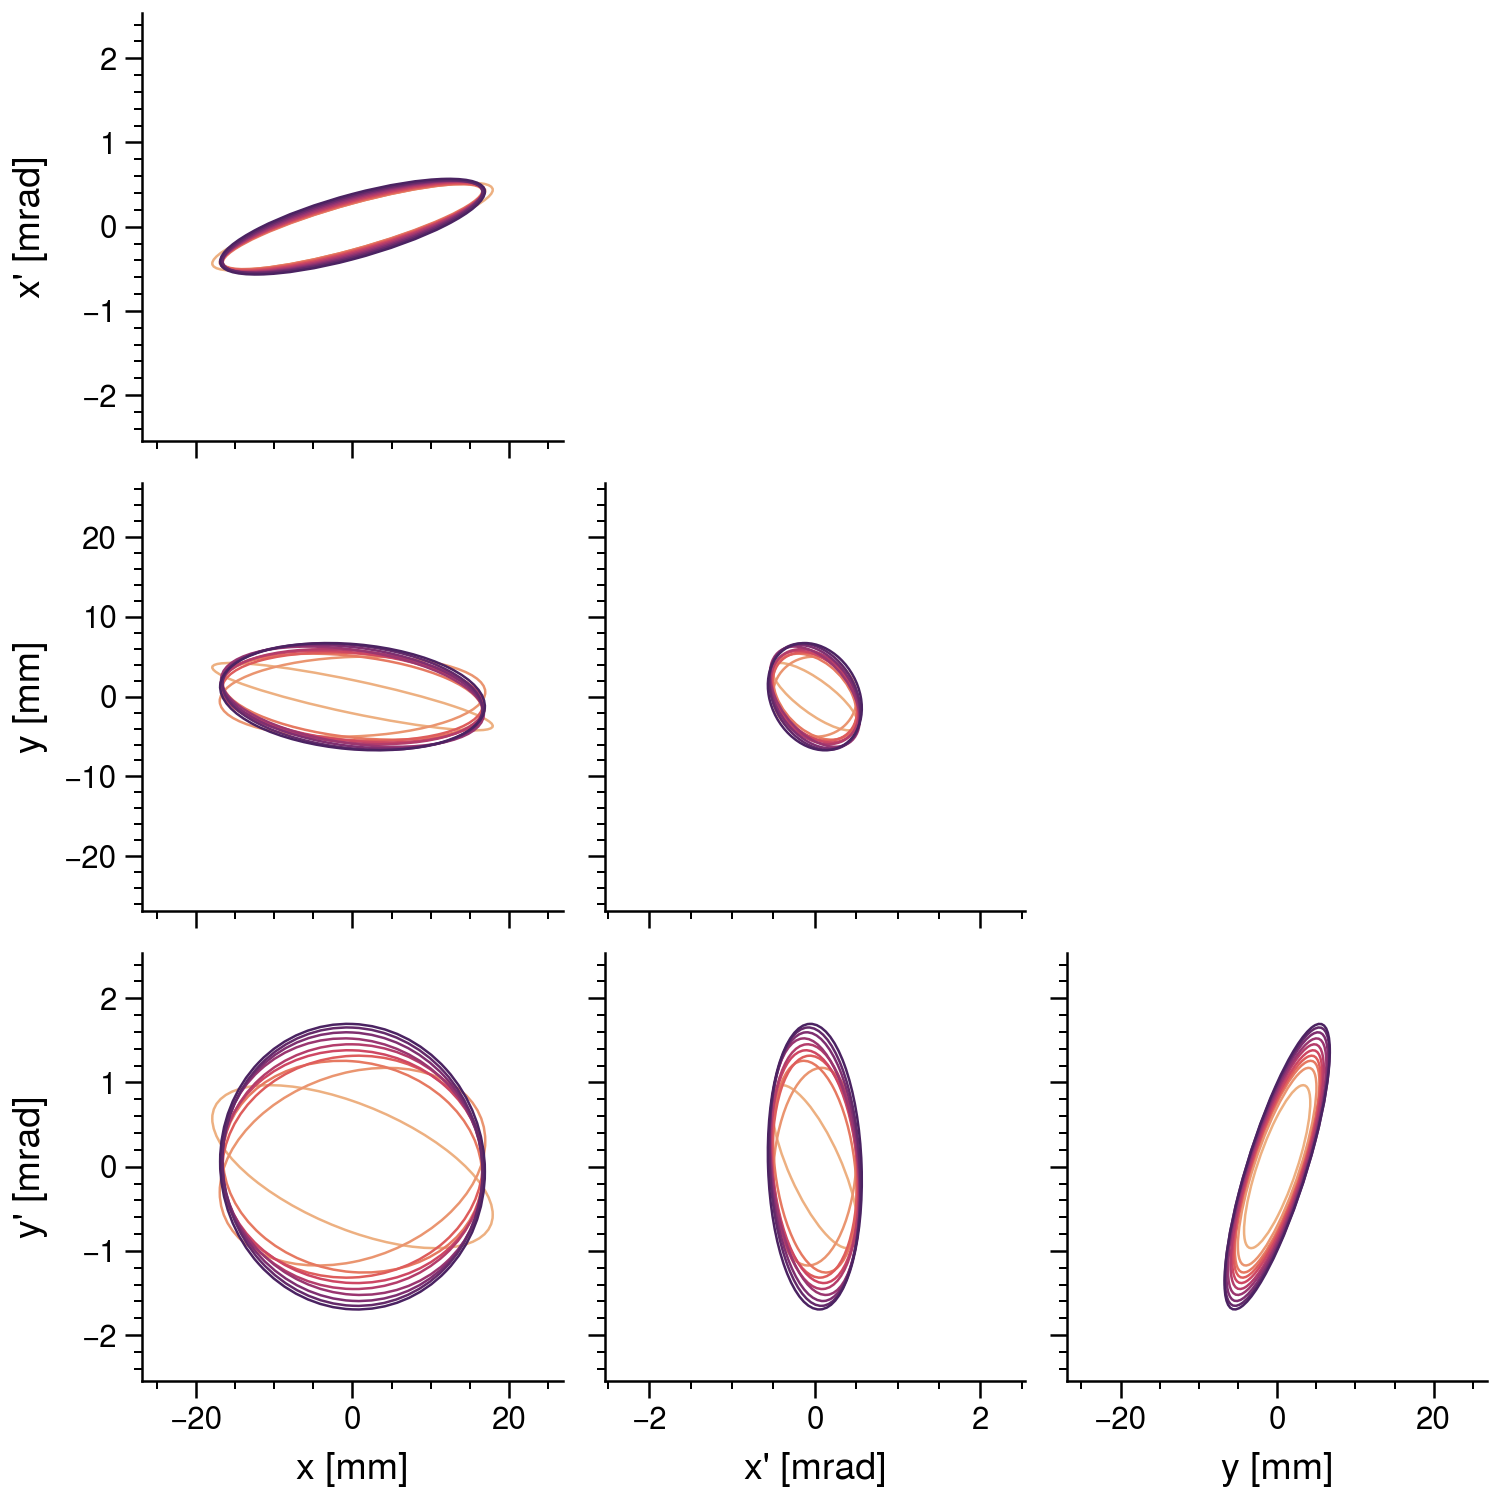
\includegraphics[width=\textwidth]{Images/chapter5/exp1b/corner.png}
    \end{subfigure}
    \hfill
    \begin{subfigure}[t]{0.39\textwidth}
        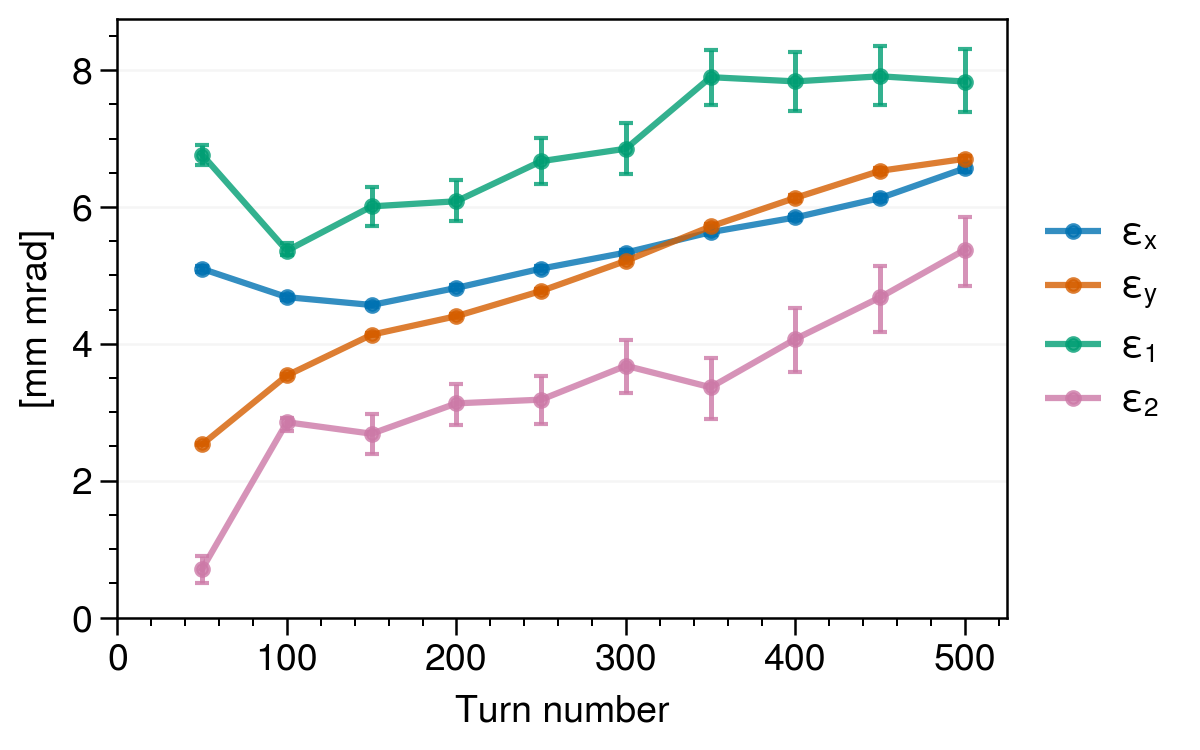
\includegraphics[width=\textwidth]{Images/chapter5/exp1b/emittances.png}
    \end{subfigure}
    \caption{Reconstructed emittances and covariance ellipses from Experiment 1b.}
    \label{fig:exp1b_emittances}
\end{figure}
%
Notice the growth of the vertical beam size in comparison with the horizontal size. The $x$-$x'$ distribution is a donut that fills in over time while also growing in radius, hence the relative lack of growth in the horizontal beam size. The vertical beam size, on the other hand, starts at a small value and increases throughout injection. Additionally, there is now a clear separation between the intrinsic emittances.

[Some thoughts: Might want to mention something about the comparison with the target images. We seem to be over-estimating the horizontal size and under-estimating the vertical size. Additionally, although the initial image is significantly tilted, the wire-scanner measurement gets the tilt angle wrong. This decreases my trust in these measurements. On the other hand, the $x$-$x'$ reconstruction has produced values that are close to the model prediction for a production beam. Also, the intrinsic emittances are a complicated function of the beam moments, so they are probably not so sensitive to these systematic errors. Maybe what we have is some systematic error in the beam size due to the small number of points in the wire-scans?]

We close with a PIC simulation of this case in Fig.~\ref{fig:exp1b_sim}. 
%
\begin{figure}[!p]
    \centering
    \begin{subfigure}{0.85\textwidth}
        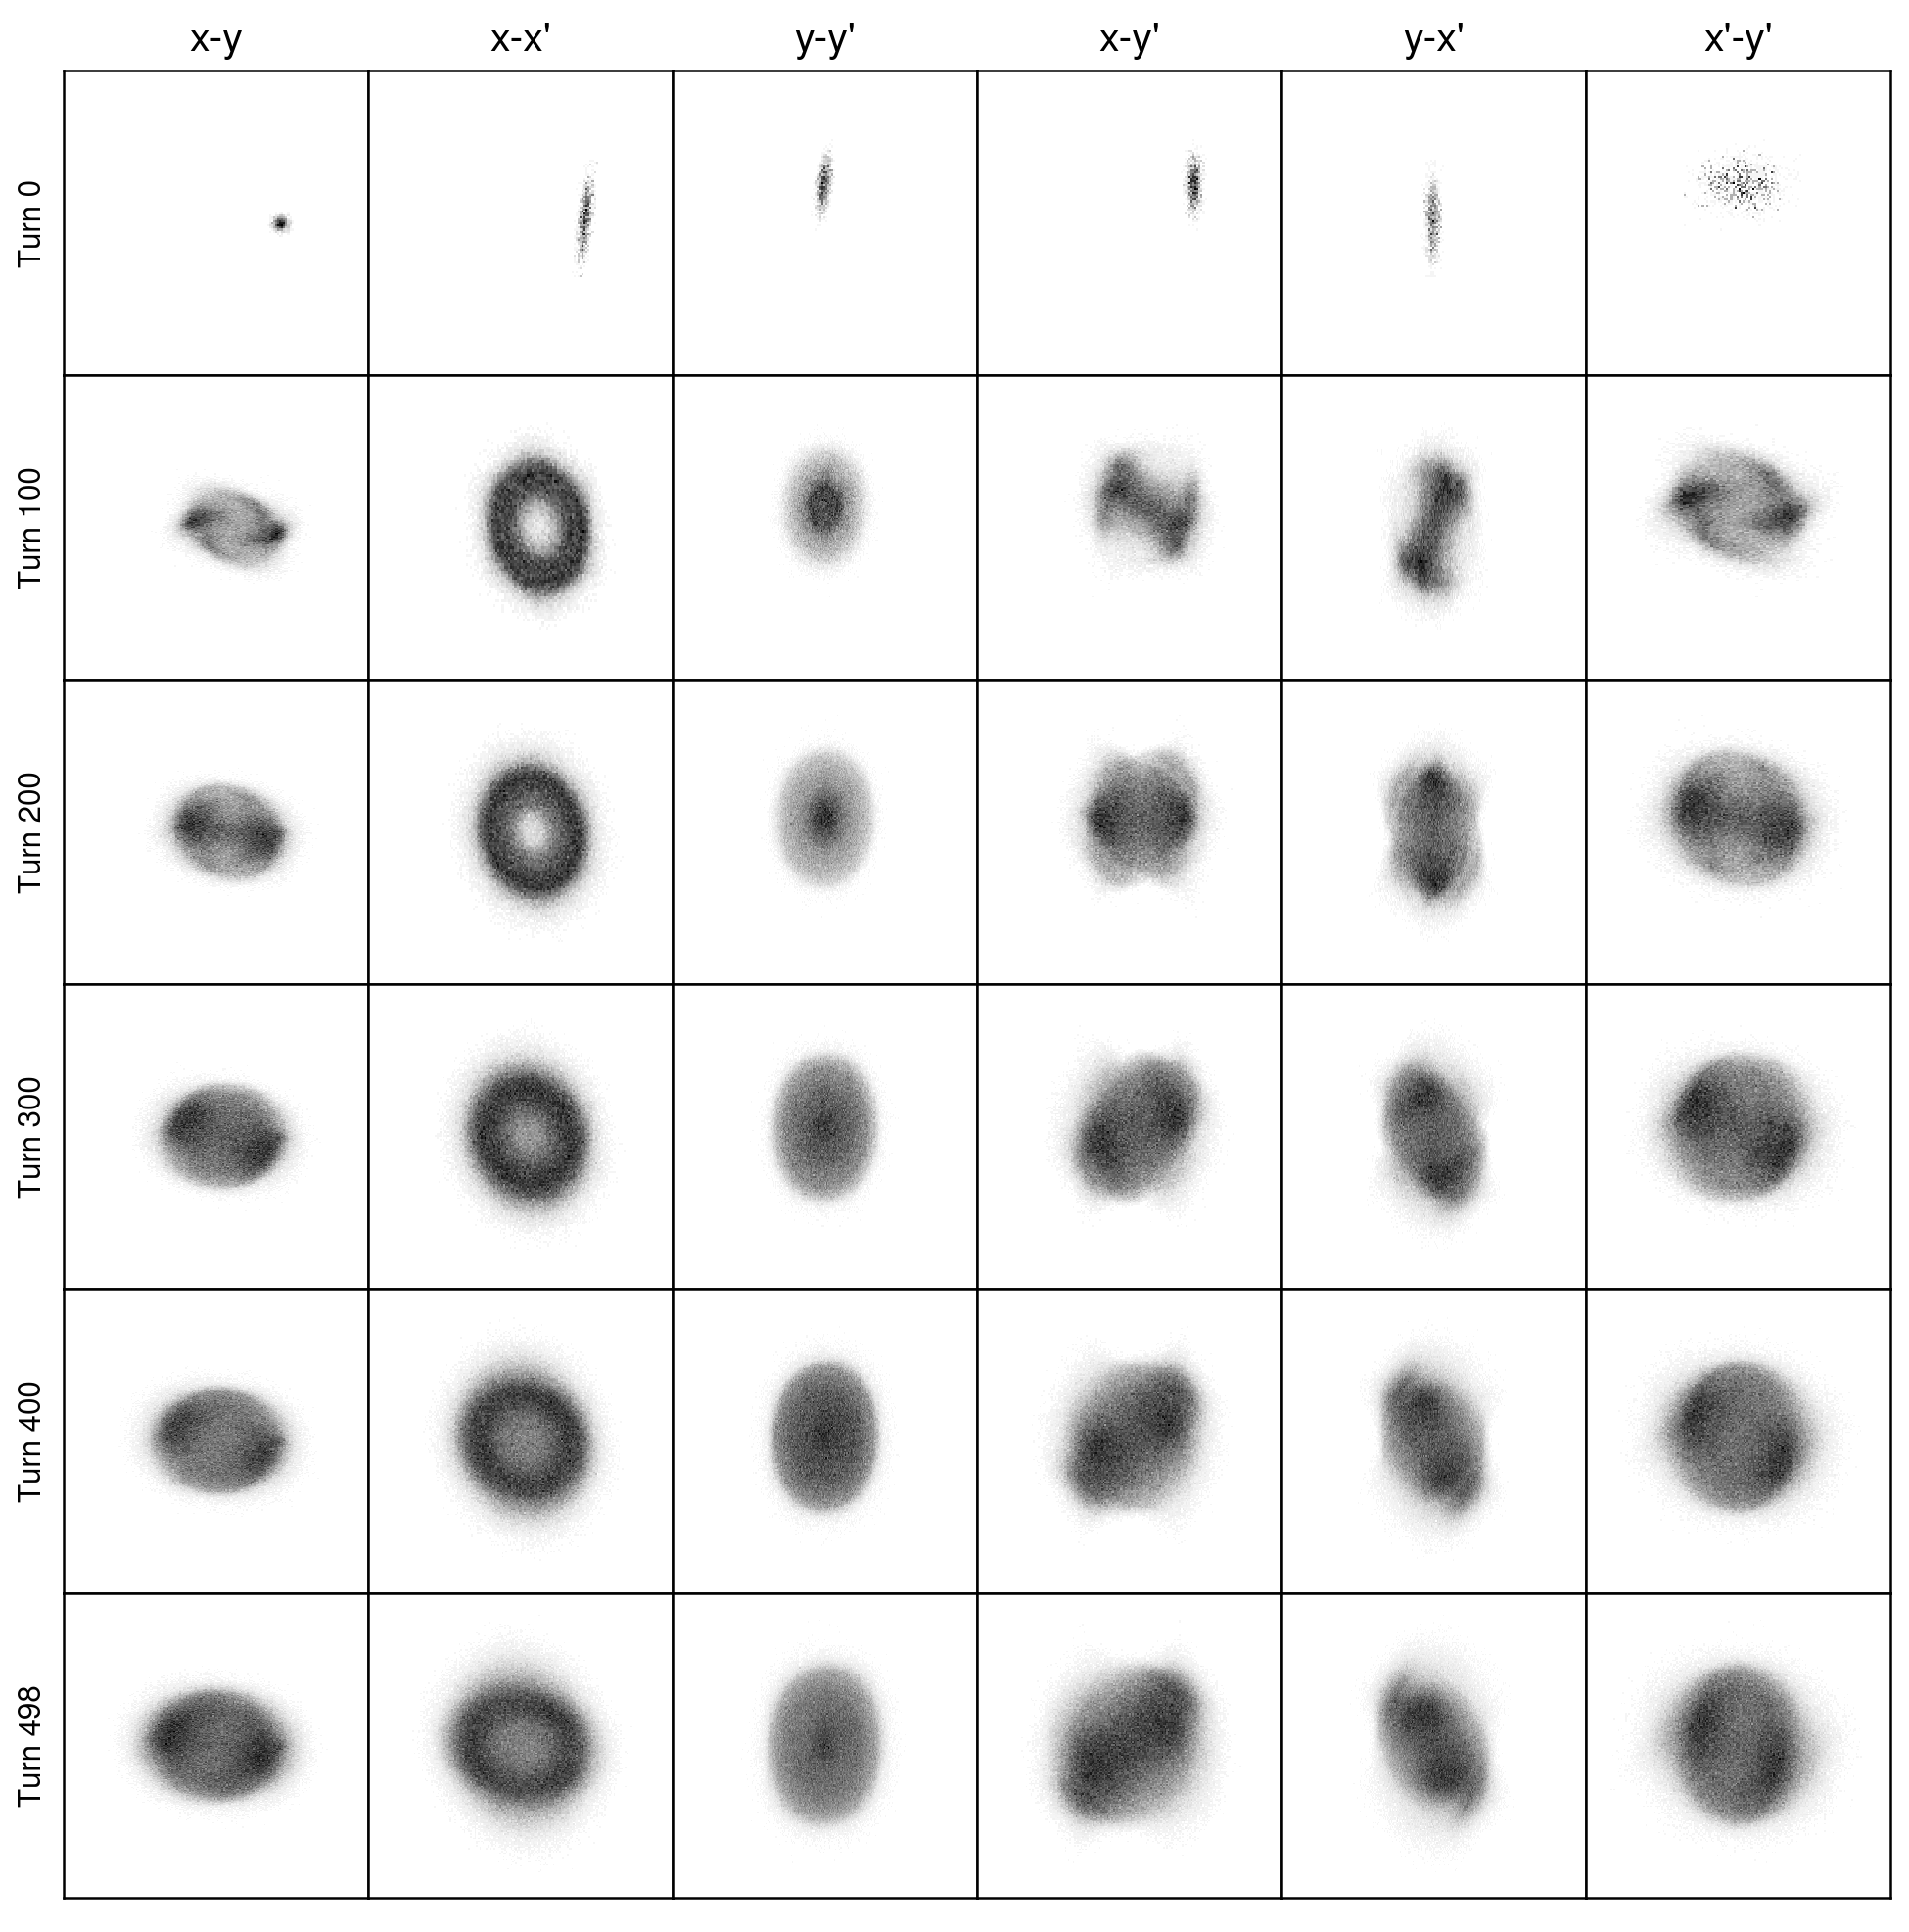
\includegraphics[width=\textwidth]{Images/chapter5/exp1b/sim_snapshots.png}
    \end{subfigure}
    \vfill
    \vspace*{1.0cm}
    \vfill
    \begin{subfigure}{0.7\textwidth}
        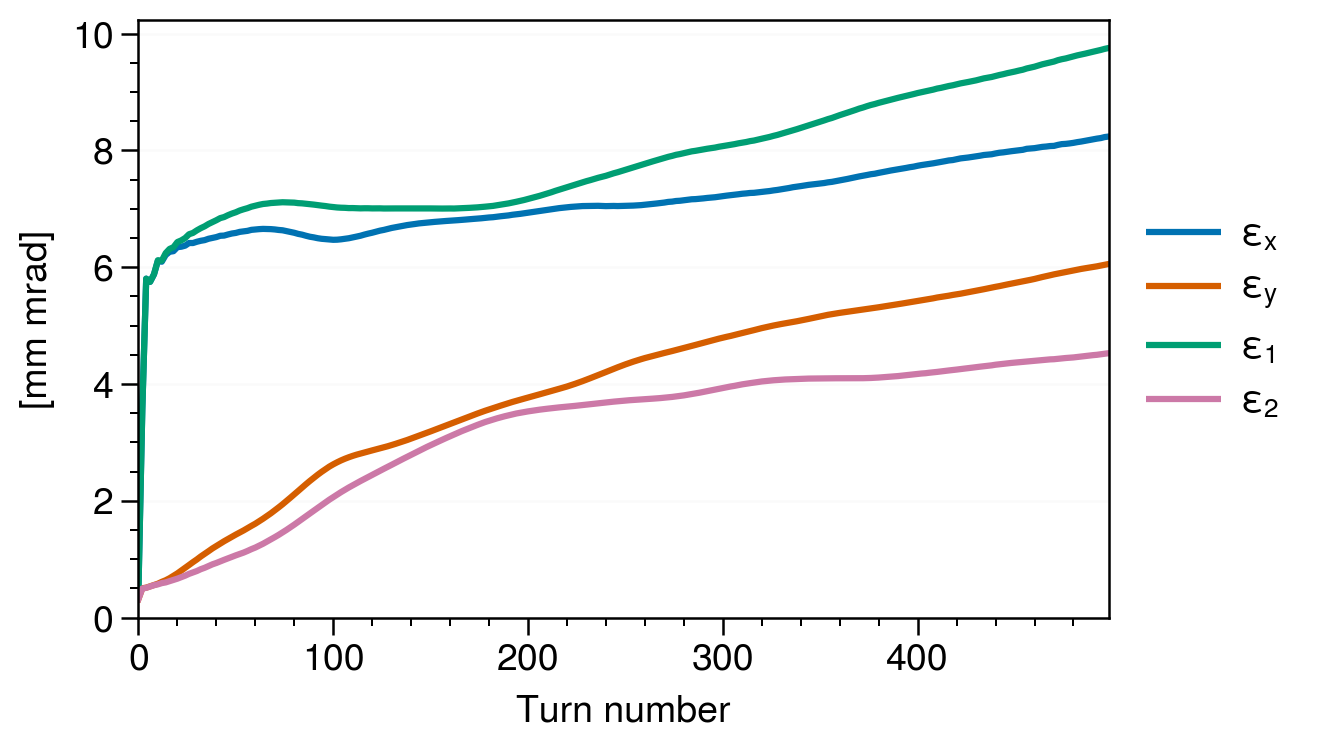
\includegraphics[width=\textwidth]{Images/chapter5/exp1b/sim_emittances.png}
    \end{subfigure}
    \caption{Simulation of experiment 1b. [RE-RUN WITH SLICED SPACE CHARGE AND TRANSVERSE IMPEDANCE. ALSO CHANGE BEAM LENGTH TO 30/64]}
    \label{fig:exp1b_sim}
\end{figure}
%
Again, keep in mind that the $\beta$ functions at the injection point are not exactly the same as in the experiment, so the absolute values of the emittances are not expected to agree. [...]




\section{Experiment 2}

In Experiment 2, the beam energy was lowered to 0.8 GeV for the first time. The closed orbit was able to reach the foil, and a maximum vertical slope of ${y'}_{max} \approx 1.1$ mrad was achieved. This is significantly smaller that the 1.7 mrad used in the simulations from \cite{Holmes2018}. 

In the setup procedure, an optional step was listed: 3. Modify the injection region in some way to assist the injection kickers. There are several tricks that can be played to increase ${y'}_{max}$. One option would be to move the foil farther into the beam pipe, but this is undesired because it would require modification of the trajectory of the surviving hydrogen ions. Another option is to use the vertical orbit corrector dipoles in the injection region to increase the maximum vertical slope. This is not straightforward in reality because the correctors are already used to flatten the orbit during neutron production.

There are two correctors before and after the foil. Our strategy was to manually change the first two correctors, then use the second two correctors and every other corrector in the ring to flatten the orbit (using an existing Orbit Correction application). There are four options for the sign of the changes applied to the first two correctors: $\uparrow\uparrow$, $\uparrow\downarrow$, $\downarrow\uparrow$, $\downarrow\downarrow$. For each option, a small change was applied to the dipole currents and the injection kickers were asked to maximize the vertical slope at the foil. This did not work; modifying the correctors lead to significnat closed-orbit waves throughout the ring that could not be flattened. The use of orbit correctors is left as a future optimization. 

The remaining free parameters are the beam intensity and the maximum horizontal position $x_{max}$. Assuming $\alpha \approx 0$ at the injection point, the ratio of painted emittances is
%
\begin{equation}
    \frac{\varepsilon_y}{\varepsilon_x} \approx 
    \beta_x \beta_y \left(\frac{{y'}_{max}}{x_{max}}\right)^2 
\end{equation}
%
It is desirable to paint equal emittances. In simulations, this can easily be achieved since the $\beta$ functions are known. In reality, the exact $\beta$ functions are unknown. The model $\beta$ functions at the injection point are both near 10 mm/mrad; for $y'_{max}$ = 1 mrad, this would require $x_{max}$ = 10 mm — a small beam. But we must keep in mind that the ratio is quite sensitive to changes in $\beta_{x, y}$; for example, $\beta_x$ = $\beta_y$ = 11 m/rad would produce $\varepsilon_y / \varepsilon_x \approx 1.5$. We decided to use $x_{max}$ = 21 mm. The beam intensity was kept at 500 injected turns, or roughly $0.75 \times 10^{14}$ protons.

The measured wire-scanner profiles are shown in Fig.~\ref{fig:exp2_wsmeas}, and the reconstructed emittances and covariance ellipses at BPM17 are shown in Fig.~\ref{fig:exp2_emittances}.
%
\begin{figure}[!p]
    \centering
    \begin{subfigure}{\textwidth}
        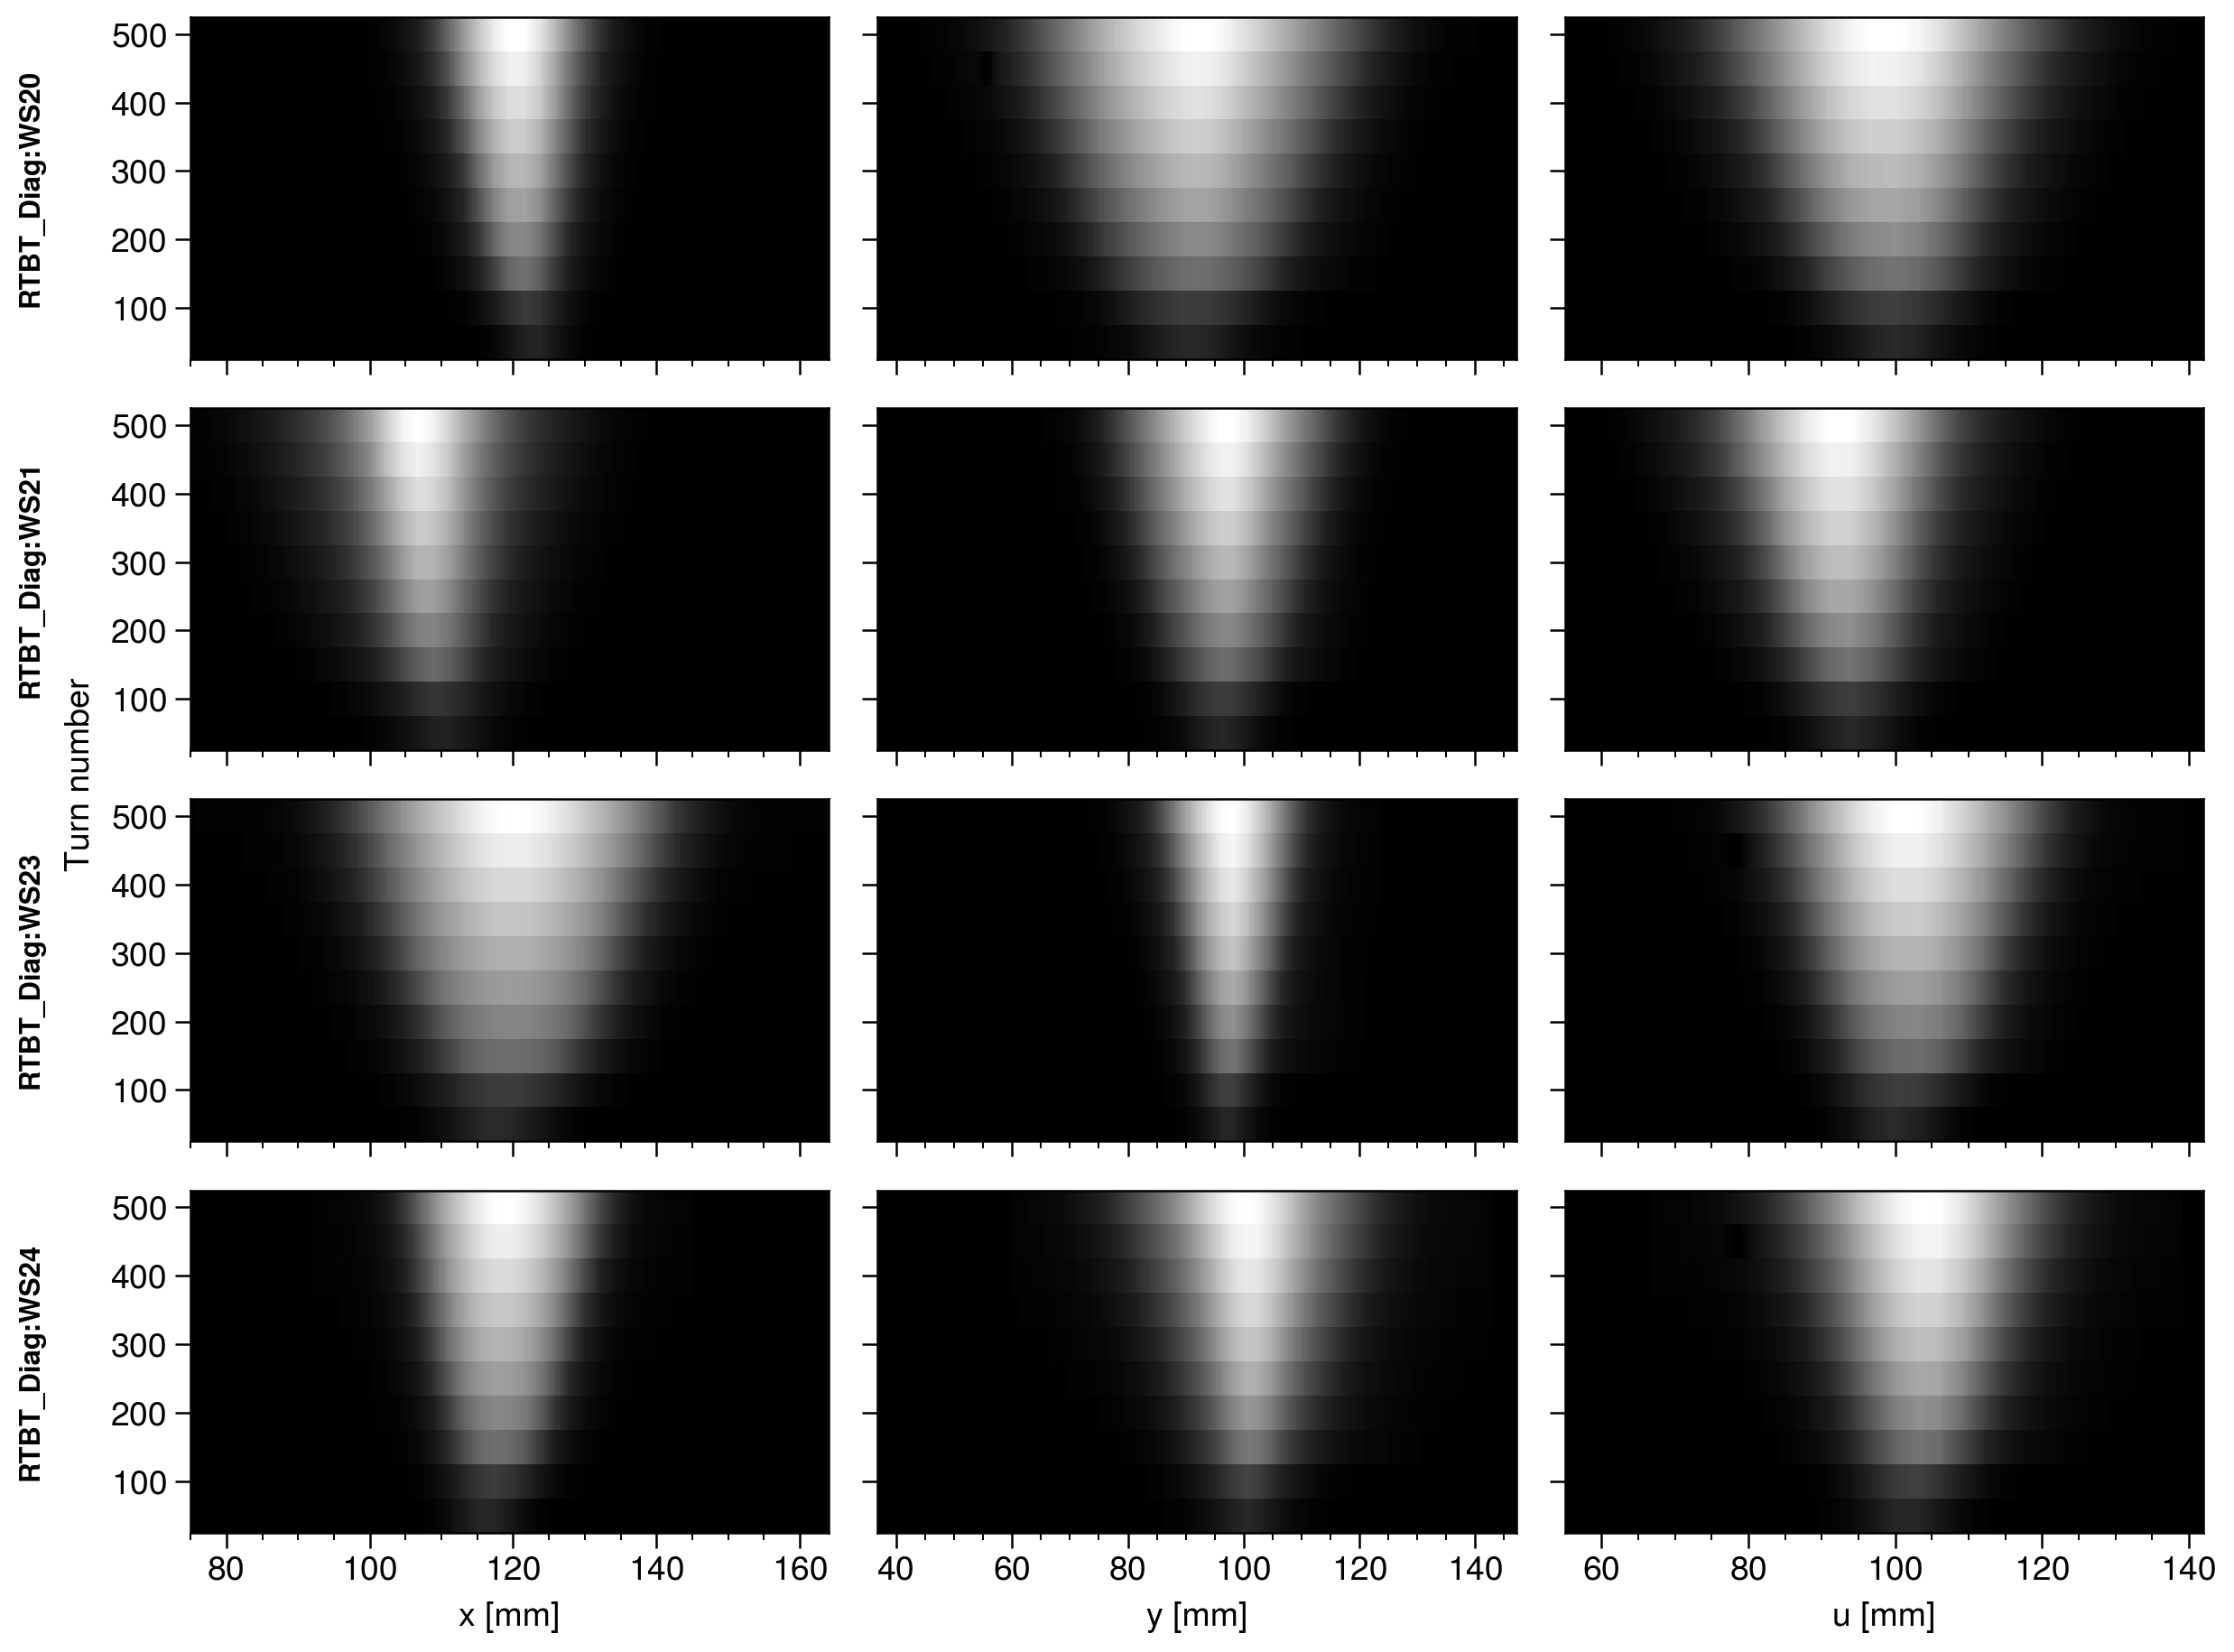
\includegraphics[width=\textwidth]{Images/chapter5/exp2/waterfall.png}
    \end{subfigure}
    \vfill
    \vspace*{1.25cm}
    \vfill
    \begin{subfigure}{\textwidth}
        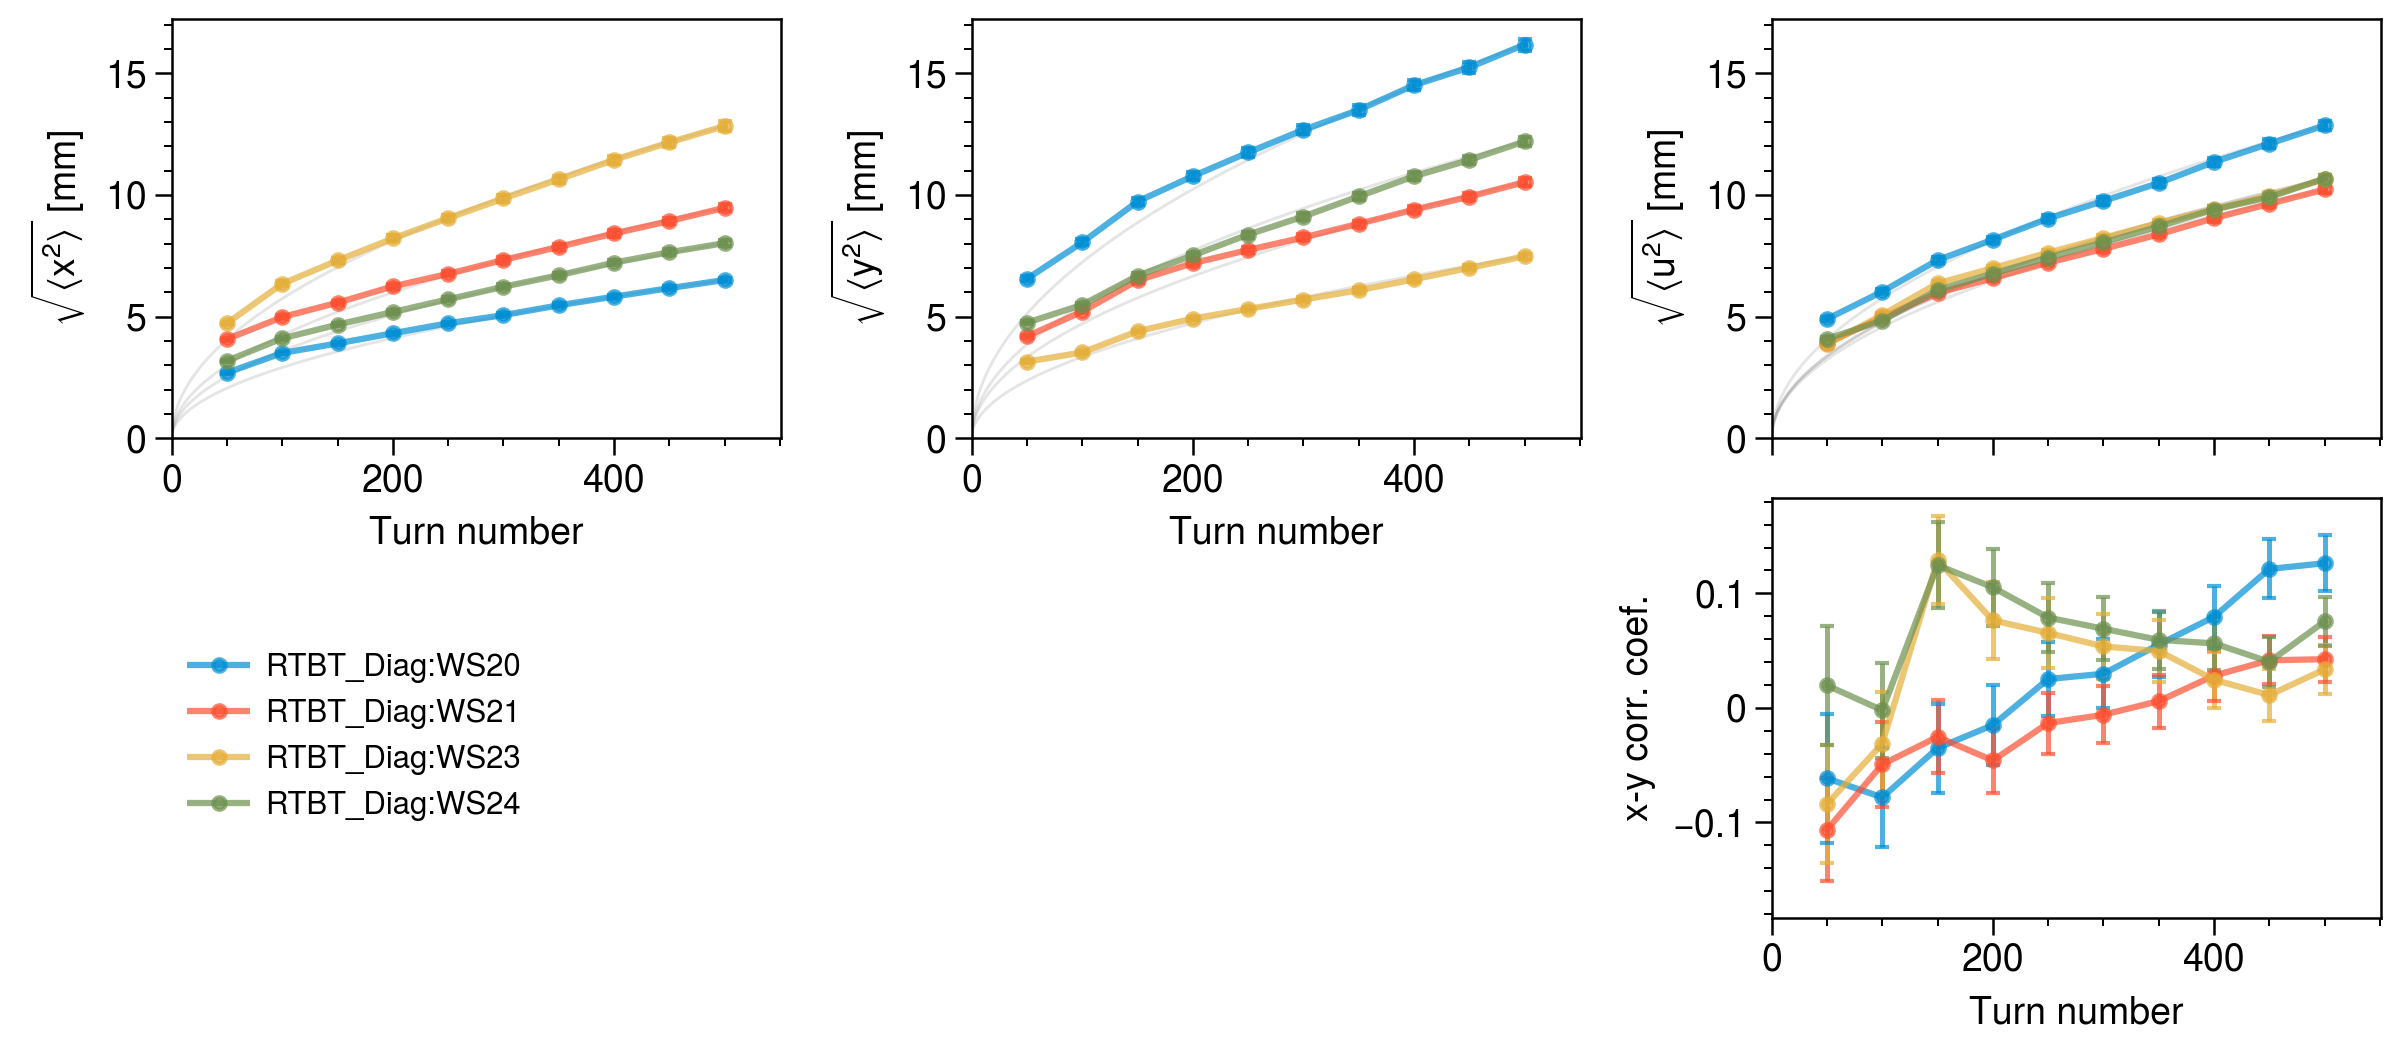
\includegraphics[width=\textwidth]{Images/chapter5/exp2/rms.png}
    \end{subfigure}
    \caption{Measured wire-scanner profiles during injection from Experiment 2.}
    \label{fig:exp2_wsmeas}
\end{figure}
%
%
\begin{figure}[!p]
    \centering
    \begin{subfigure}{0.6\textwidth}
        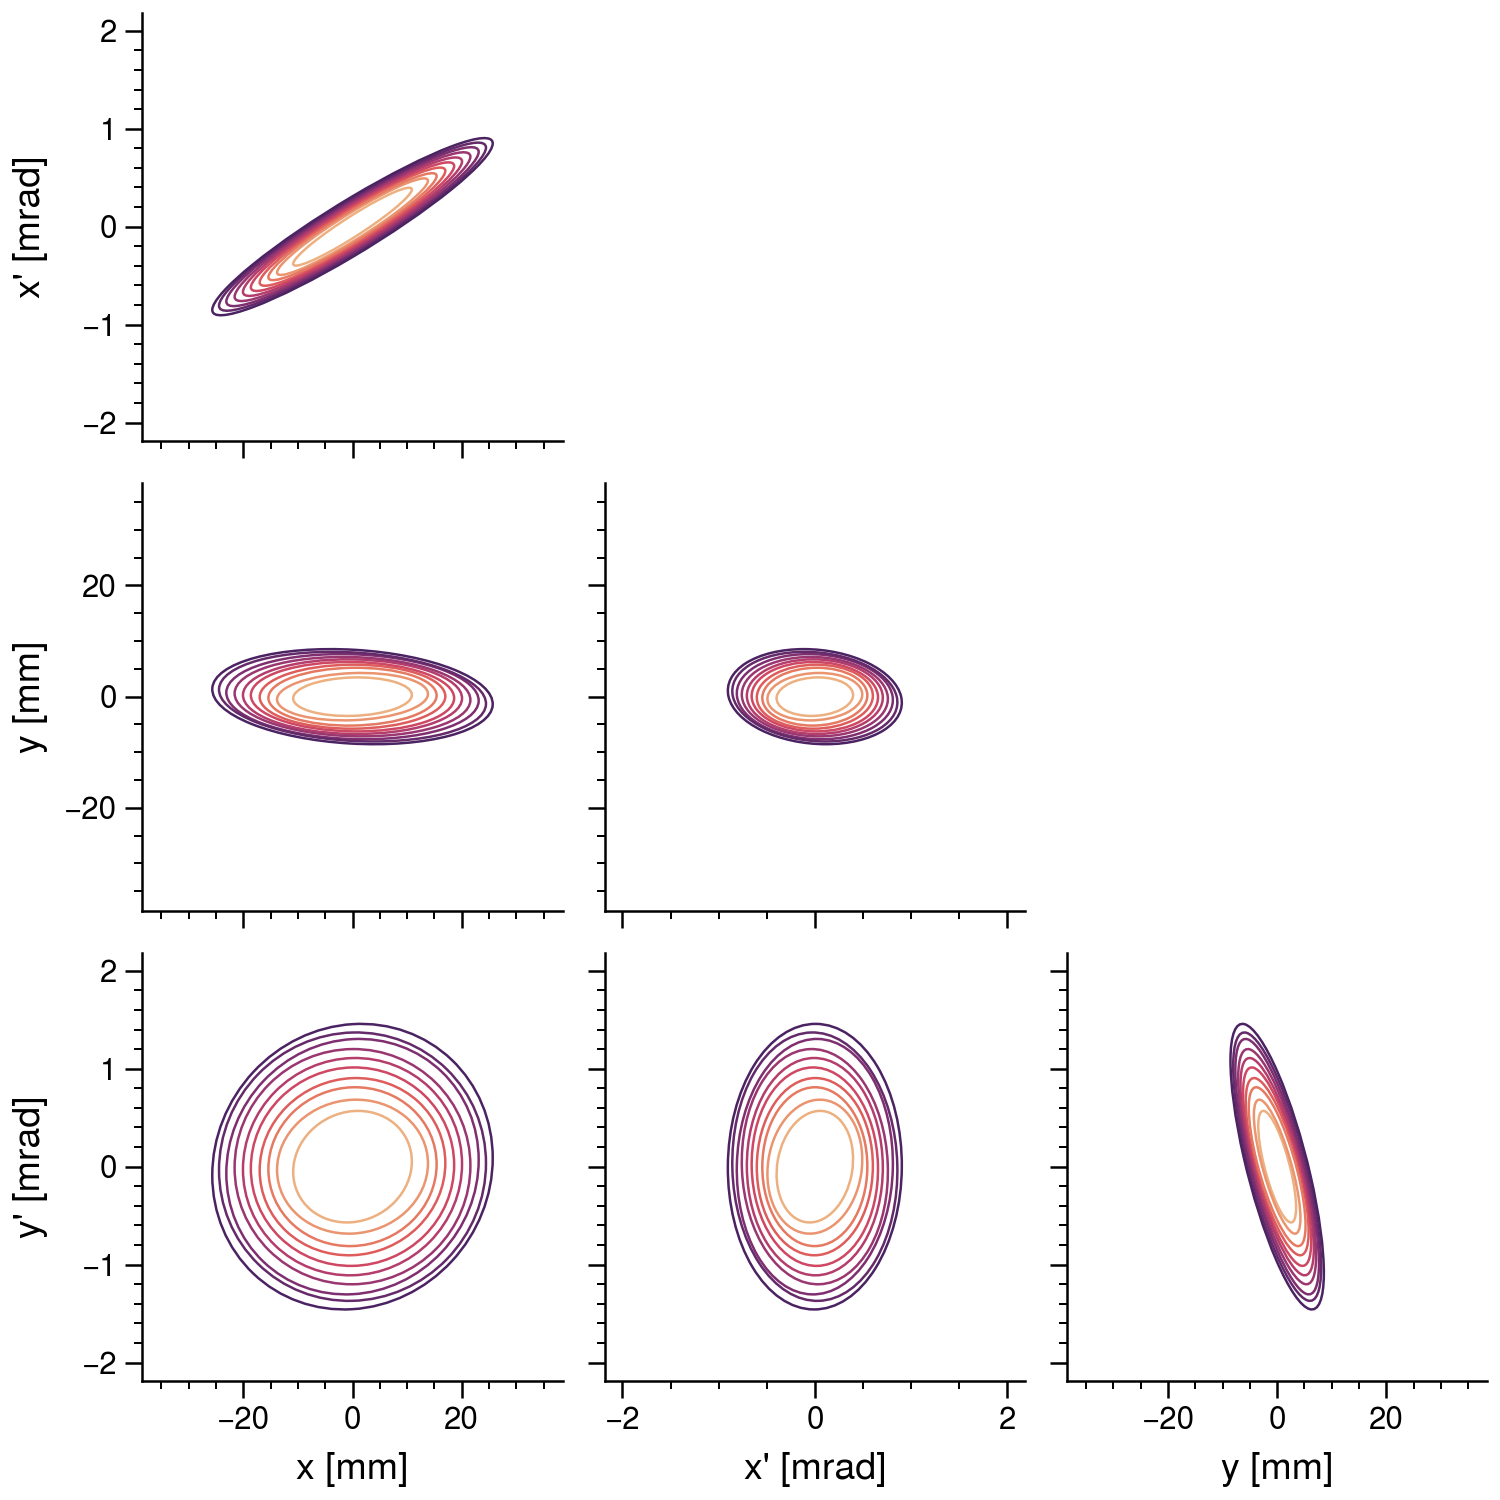
\includegraphics[width=\textwidth]{Images/chapter5/exp2/corner.png}
    \end{subfigure}
    \hfill
    \begin{subfigure}[t]{0.39\textwidth}
        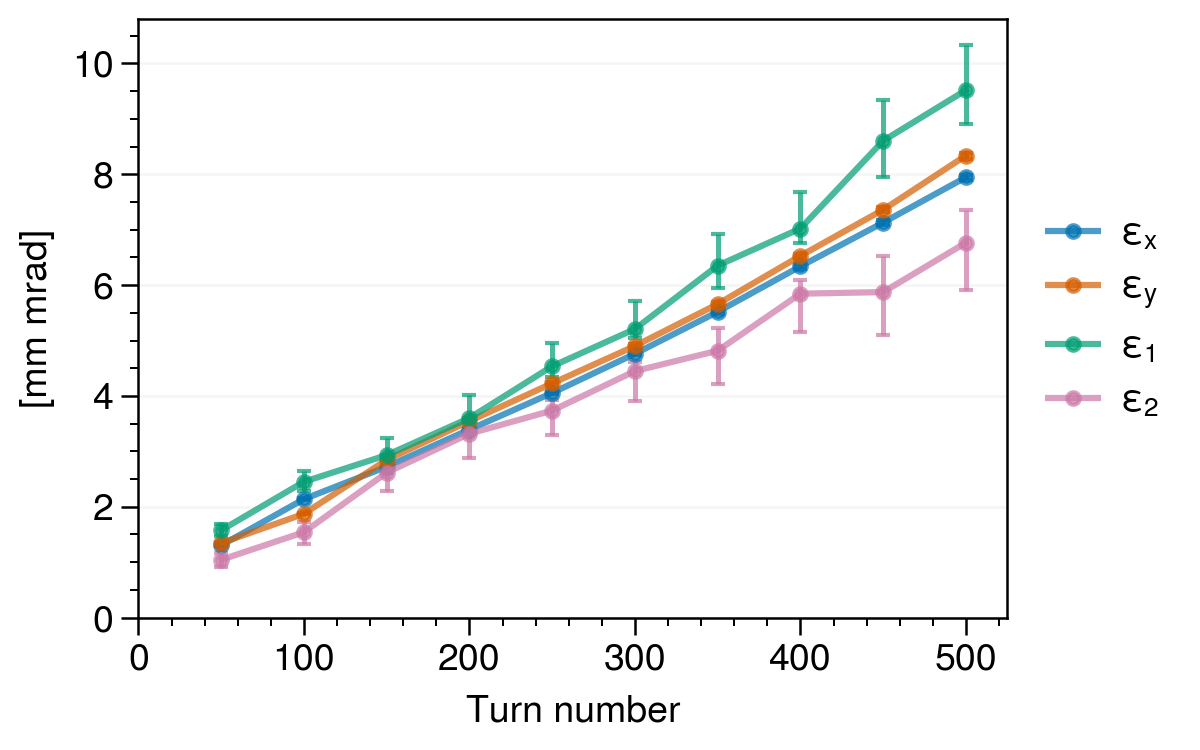
\includegraphics[width=\textwidth]{Images/chapter5/exp2/emittances.png}
    \end{subfigure}
    \caption{Reconstructed emittances and covariance ellipses from Experiment 2.}
    \label{fig:exp2_emittances}
\end{figure}
%
The apparent emittances increase linearly from a small initial value, as desired. The intrinsic emittances begin to split, although not by much, at the end of injection.

A simulation of this case is shown in Fig.~\ref{fig:exp2_sim}.
%
\begin{figure}[!p]
    \centering
    \begin{subfigure}{0.85\textwidth}
        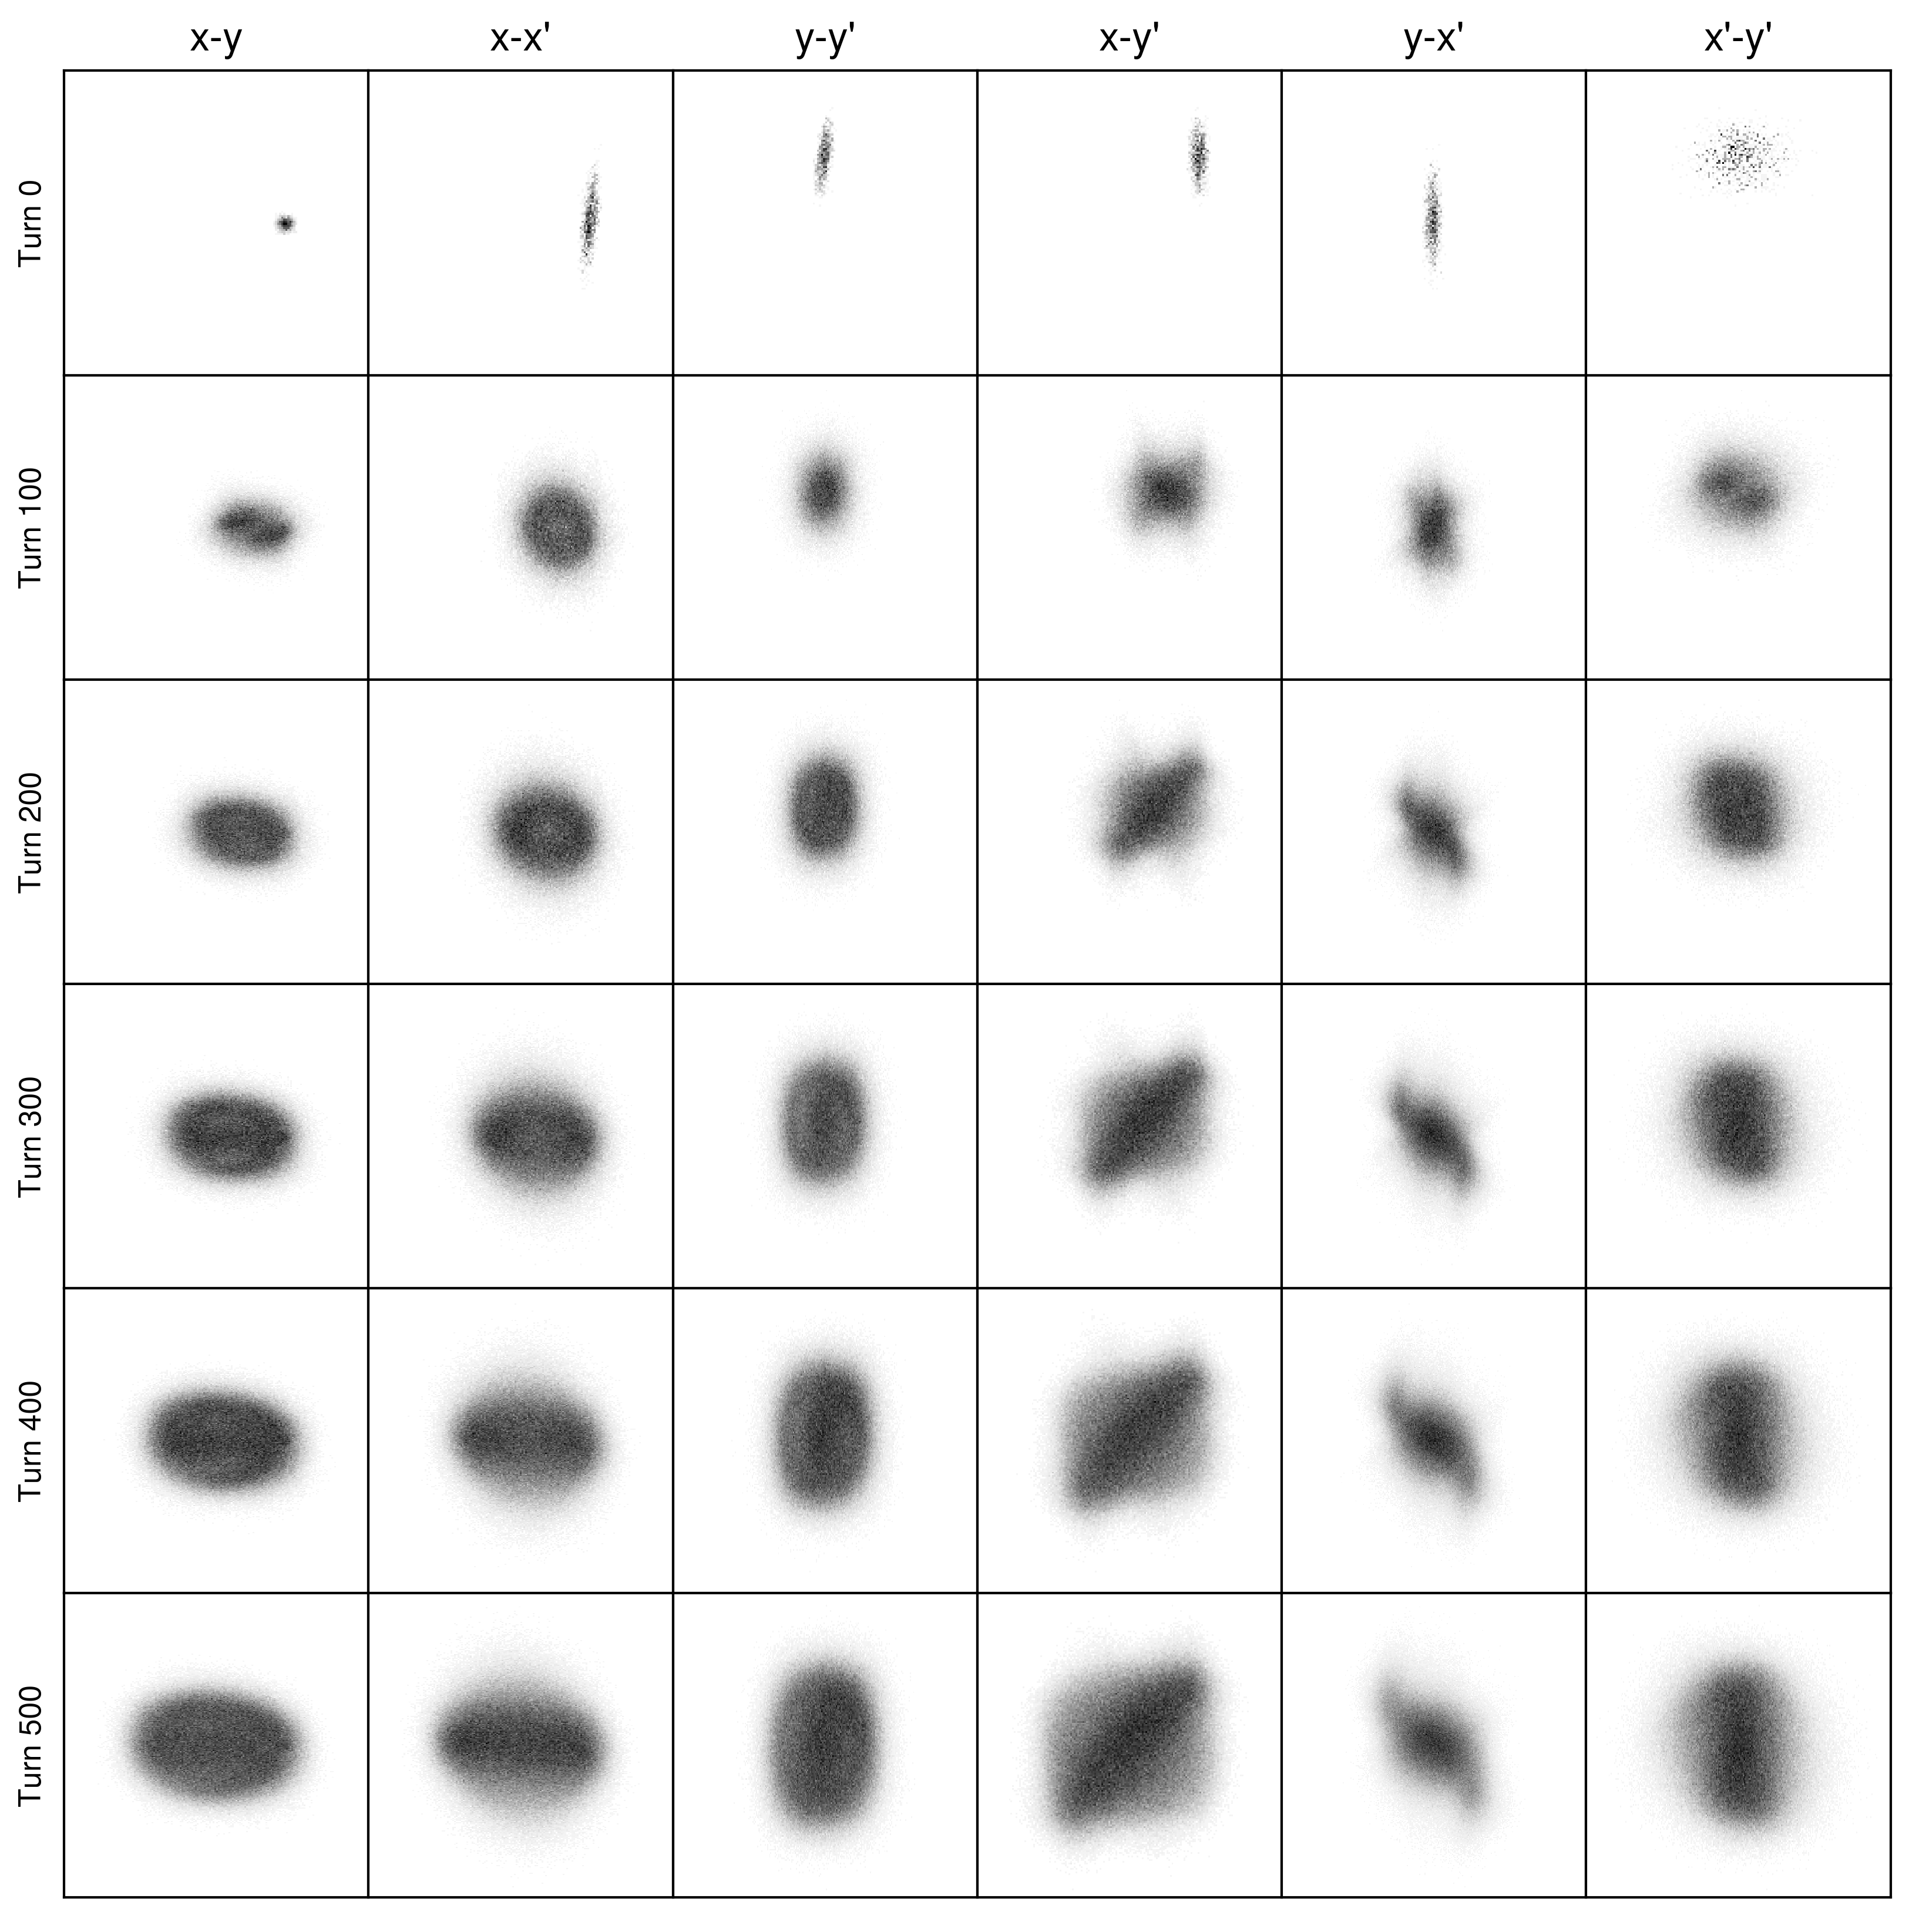
\includegraphics[width=\textwidth]{Images/chapter5/exp2/sim_snapshots.png}
    \end{subfigure}
    \vfill
    \vspace*{1.0cm}
    \vfill
    \begin{subfigure}{0.7\textwidth}
        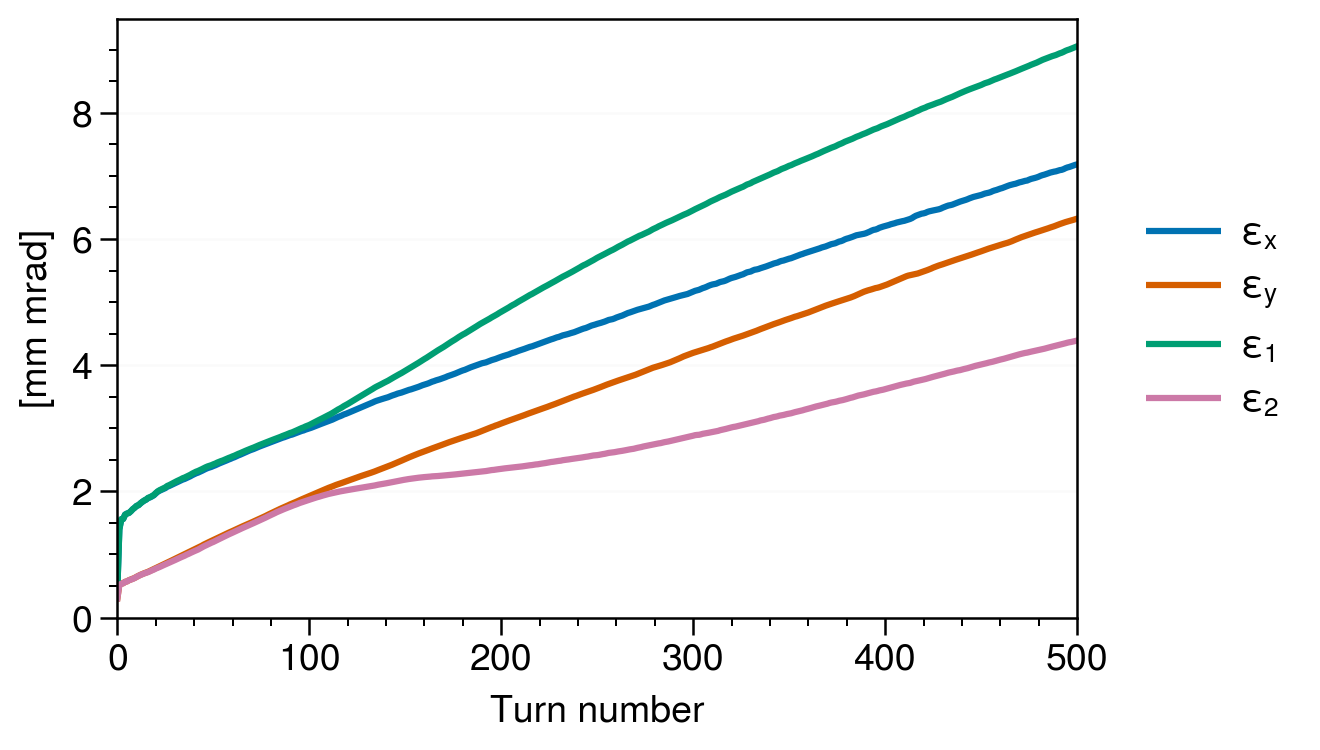
\includegraphics[width=\textwidth]{Images/chapter5/exp2/sim_emittances.png}
    \end{subfigure}
    \caption{Simulation of experiment 2.}
    \label{fig:exp2_sim}
\end{figure}
%
Notice that $\varepsilon_2$ begins to flatten after turn 100, but does not remain flat. Although the final $x$-$y'$ projection has a higher density along the painting path, the linear correlation is significantly blurred. This is likely because space charge has a strong effect on the evolution at this intensity, energy, and beam size. Nonetheless, the simulation predicts a "better" result than what was measured.



\section{Experiment 3}

The same setup for Experiment 2 was repeated in Experiment 3. One difference was that the beam length was increased from roughly 30/64 of the ring length to 45/64 of the ring length to better approximate a coasting beam. At the start of the experiment, the beam intensity and beam size were varied; at each setting, the emittances of the final distribution were reconstructed using four wire-scanner profiles. The results are shown in Fig.~\ref{fig:exp3_search}. (The intensities are not exact; they are obtained by multiplying the nominal minipulse intensity by the number of injected turns.) Space charge clearly has an effect on the final distribution. It is somewhat surprising that the split in the intrinsic emittances increased with the beam intensity. 
%
\begin{figure}[!p]
    \centering
    \vspace*{1.0cm}
    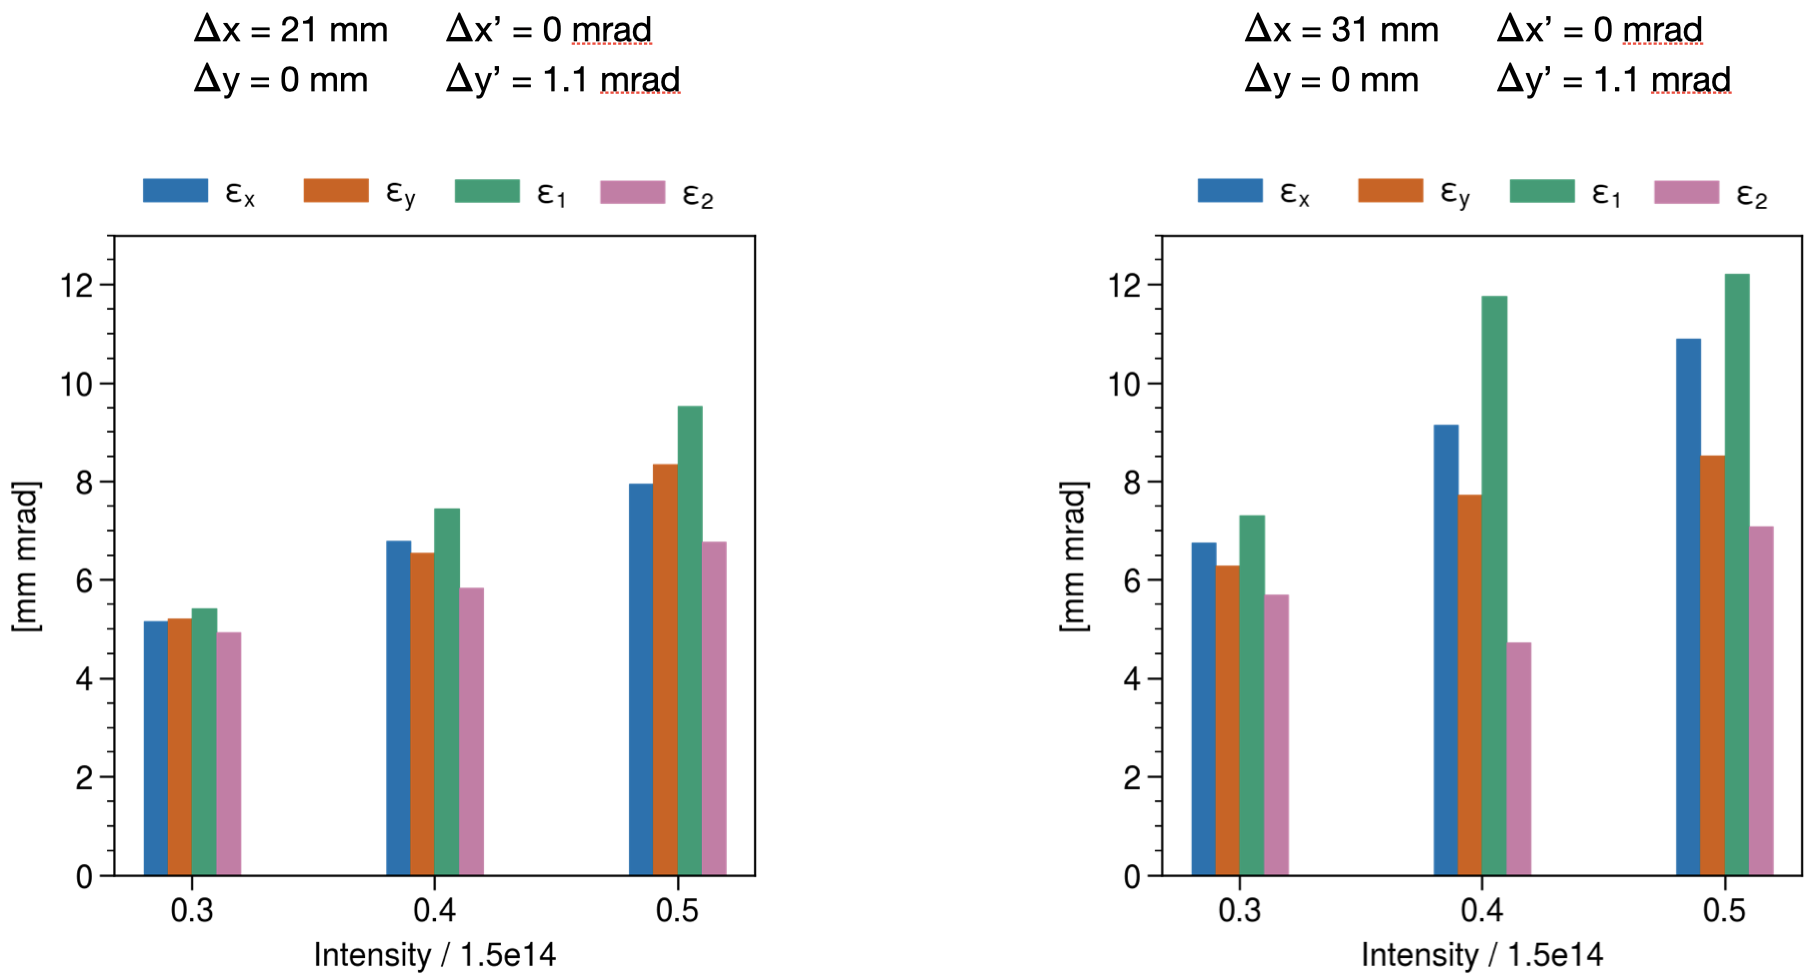
\includegraphics[width=\textwidth]{Images/chapter5/exp3/search.png}
    \caption{Measured emittances vs. beam intensity for two sets of injected coordinates.}
    \label{fig:exp3_search}
    \vspace*{1.0cm}
\end{figure}
%
The middle cluster in the right subplot was identified as the most interesting case, and the measurement process of the  of the previous two experiments were repeated — see Fig.~\ref{fig:exp3_wsmeas} and Fig.~\ref{fig:exp3_emittances}.
%
\begin{figure}[!p]
    \centering
    \begin{subfigure}{\textwidth}
        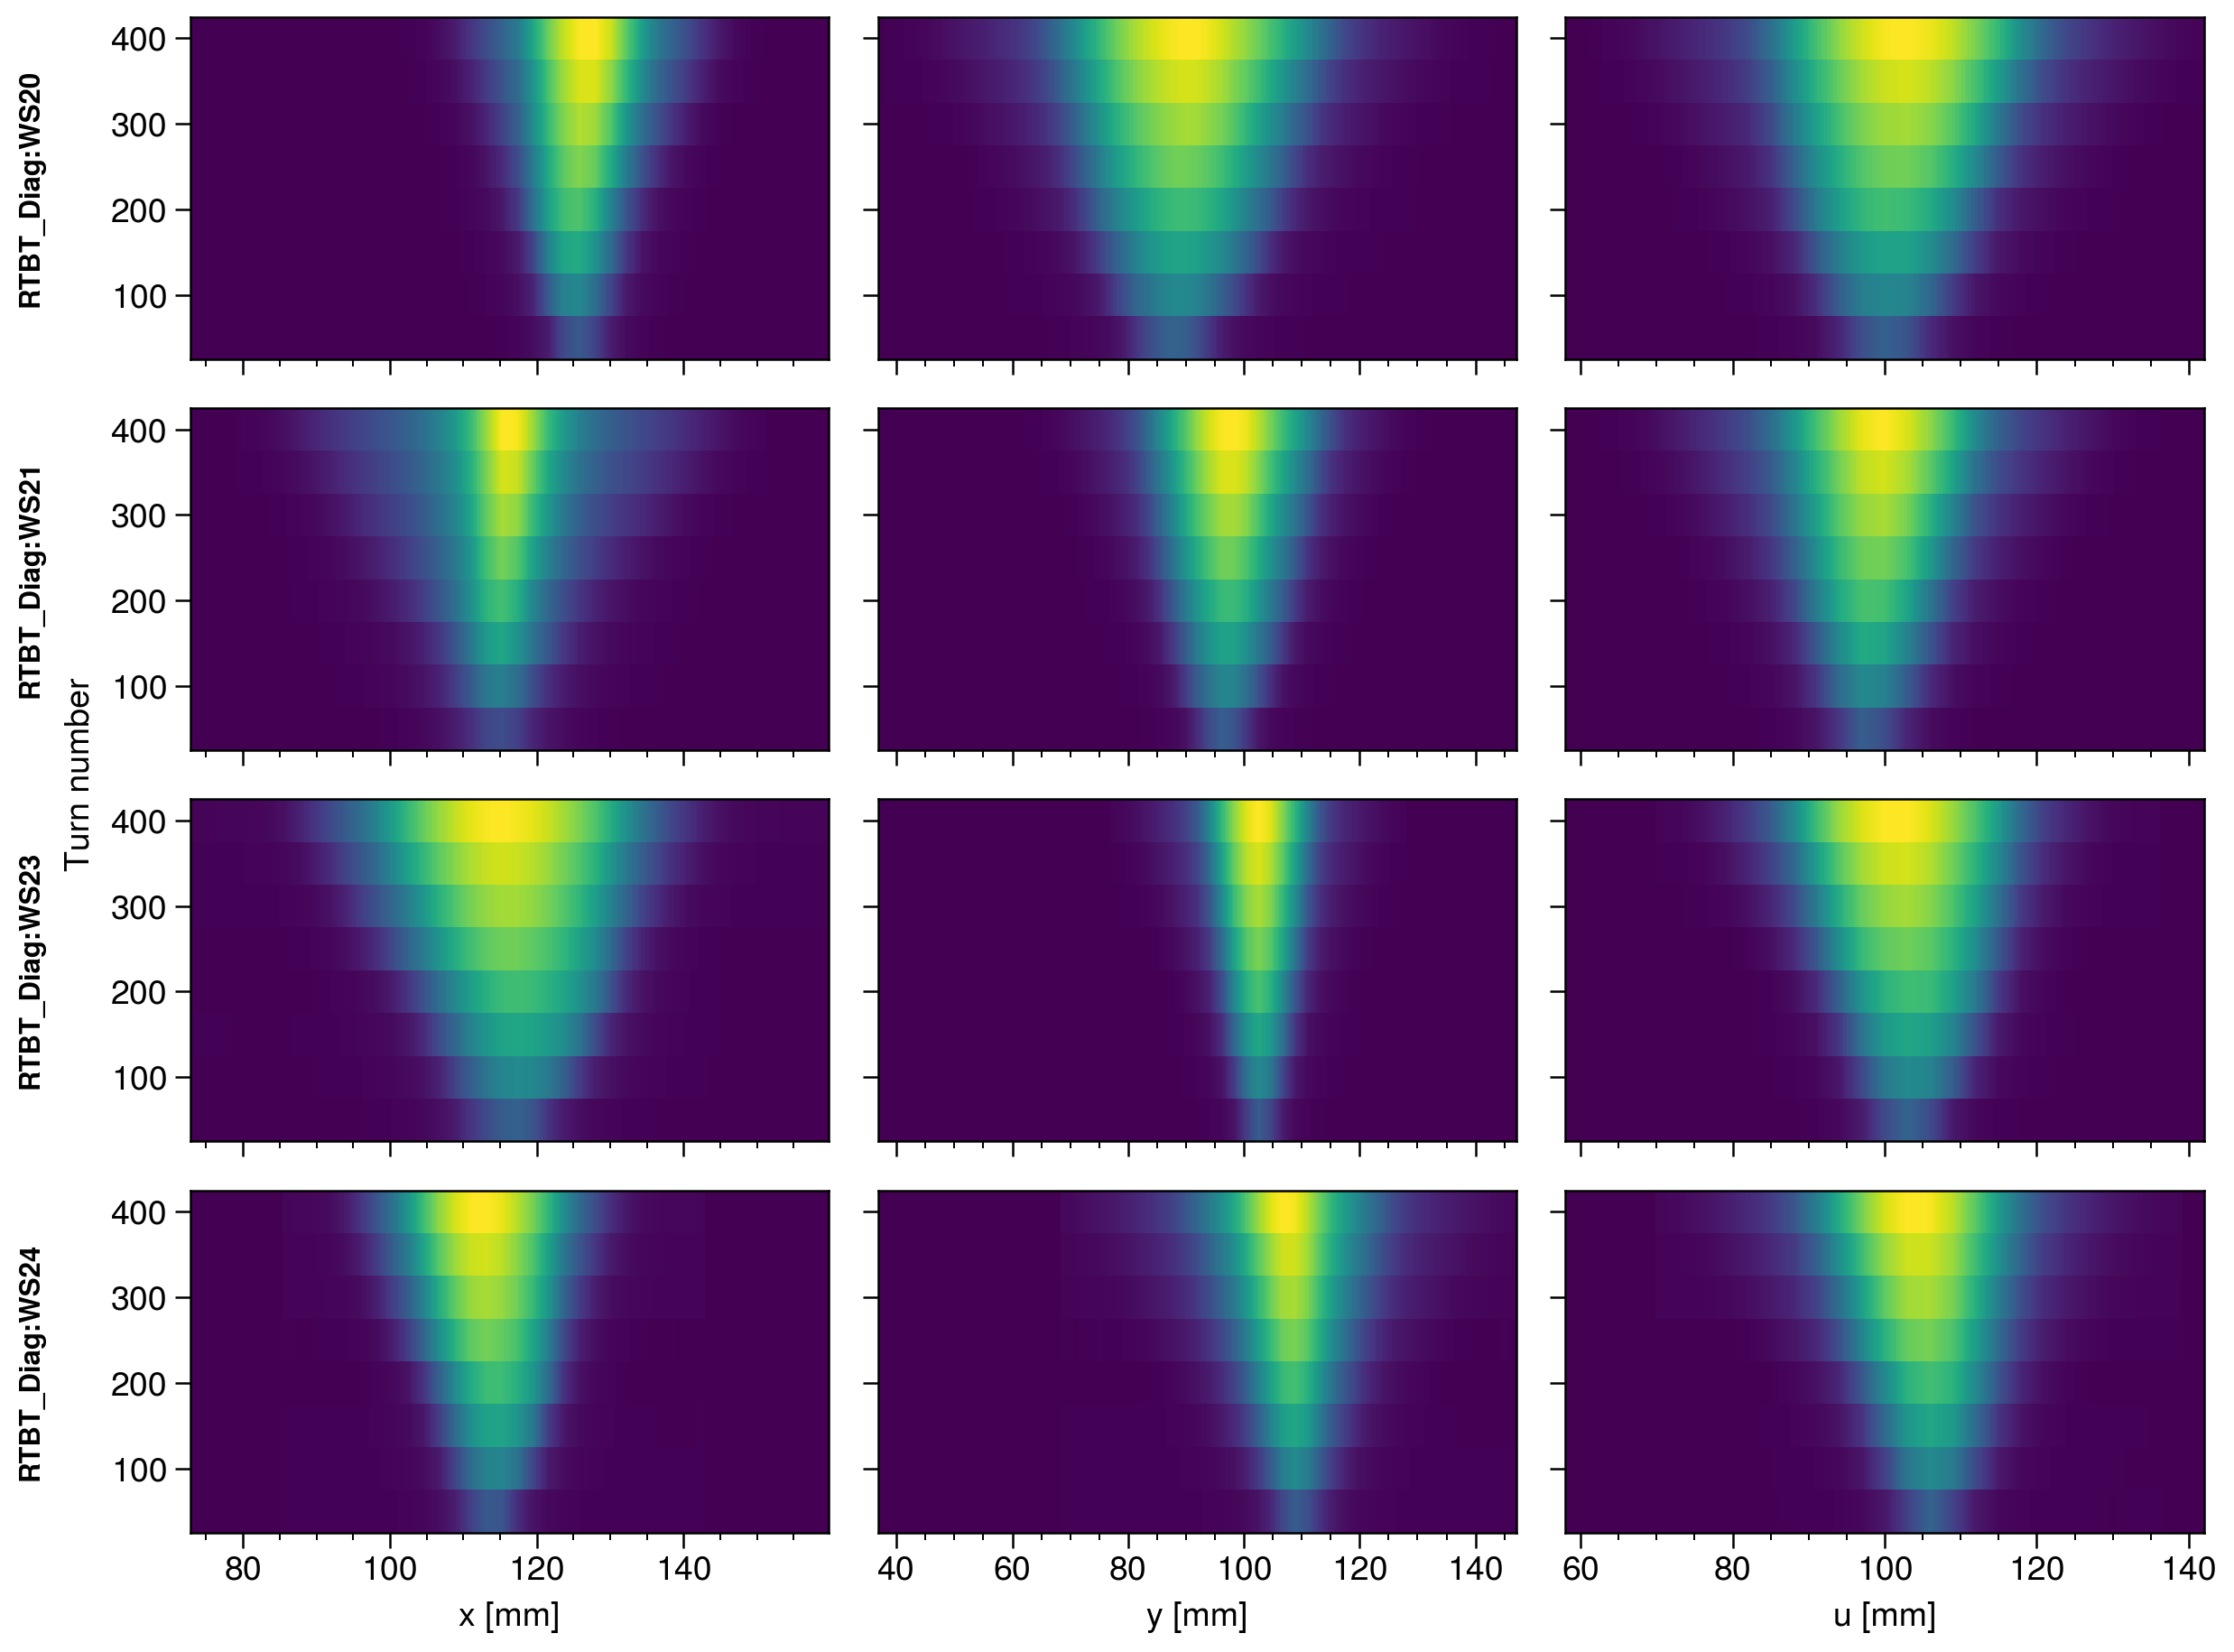
\includegraphics[width=\textwidth]{Images/chapter5/exp3/waterfall.png}
    \end{subfigure}
    \vfill
    \vspace*{1.25cm}
    \vfill
    \begin{subfigure}{\textwidth}
        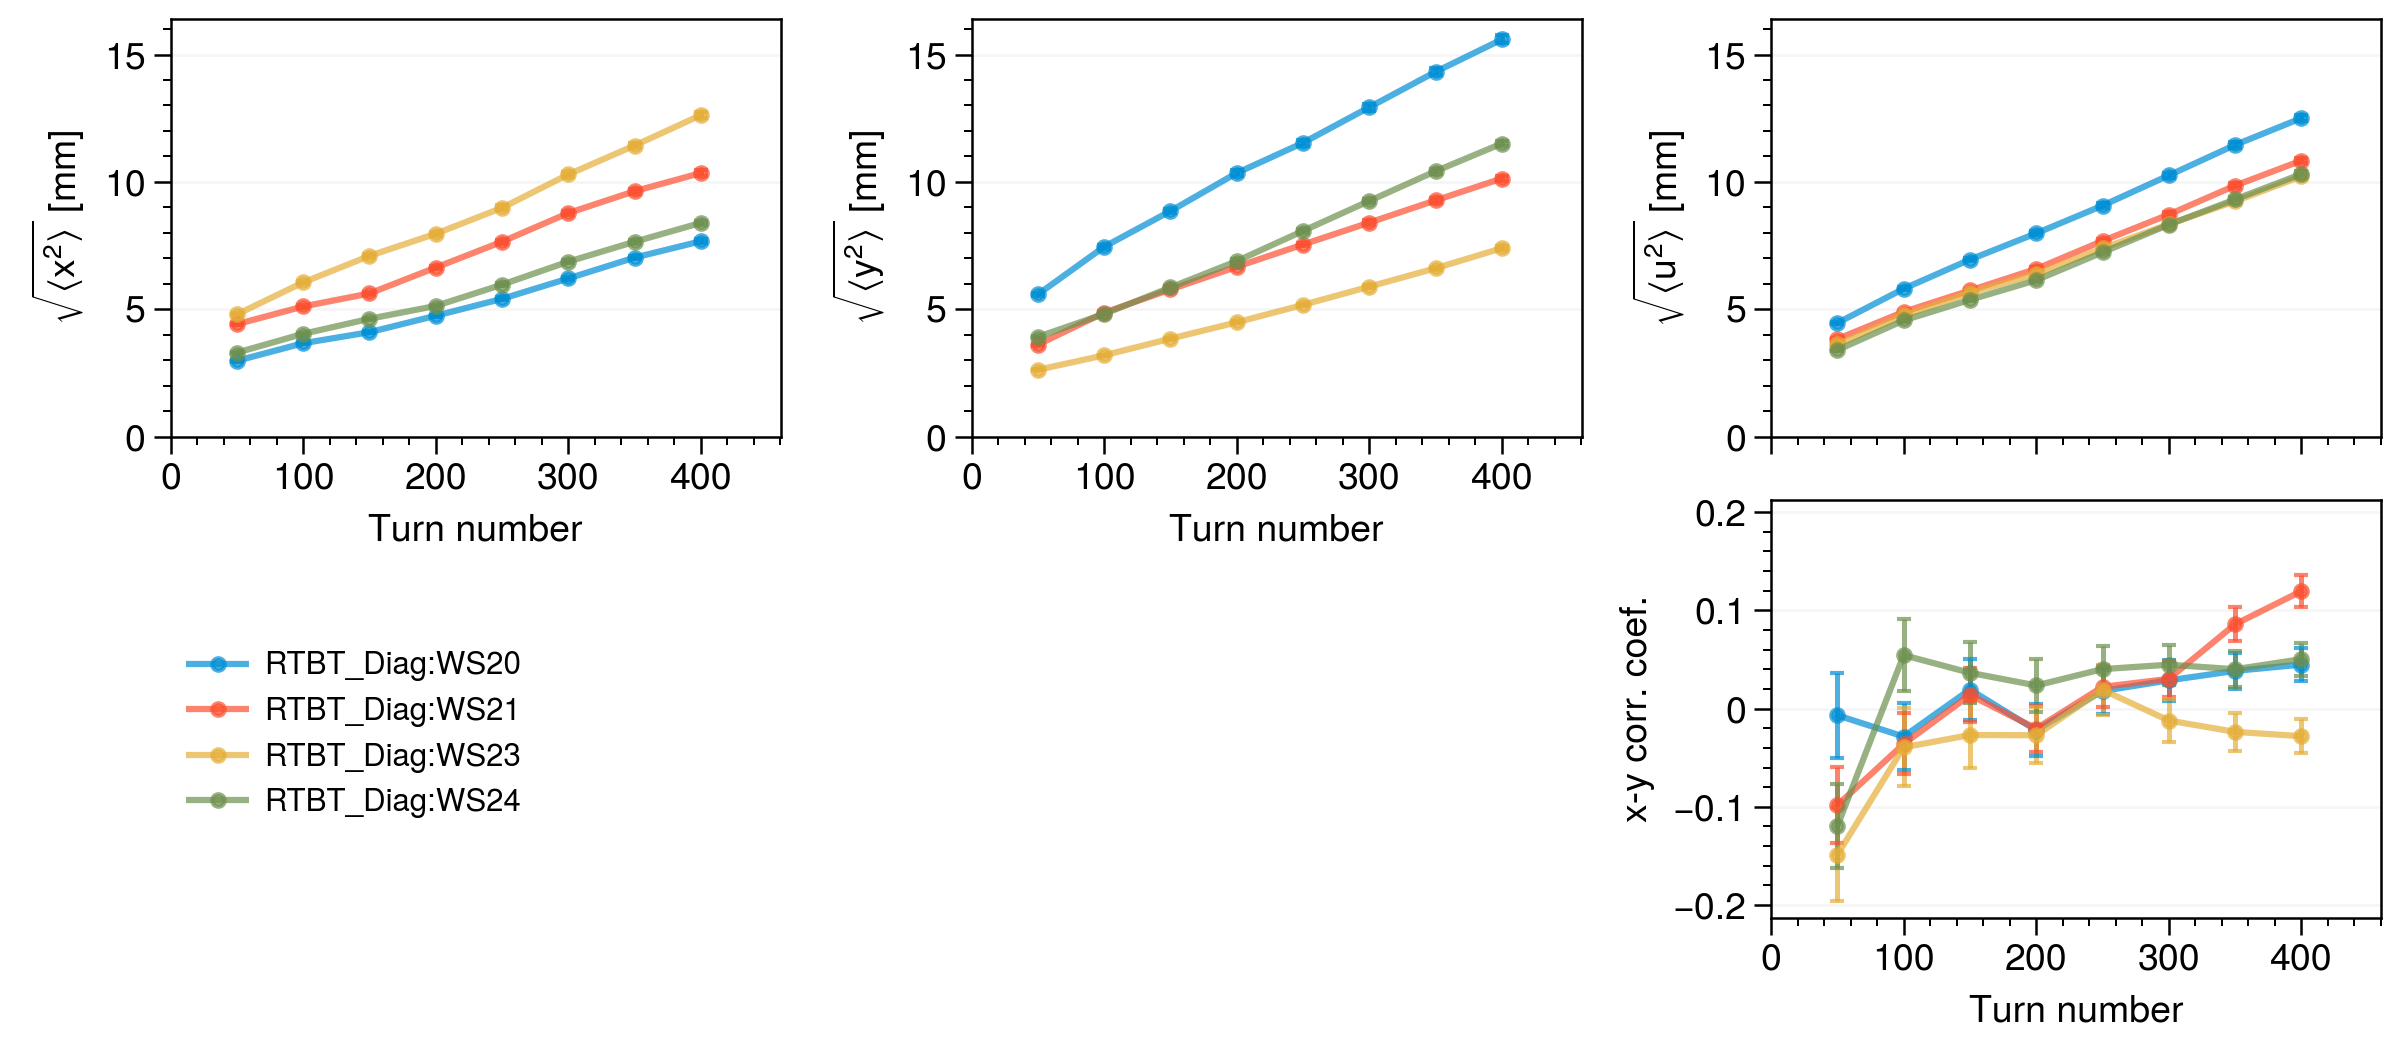
\includegraphics[width=\textwidth]{Images/chapter5/exp3/rms.png}
    \end{subfigure}
    \caption{Measured wire-scanner profiles from Experiment 3.}
    \label{fig:exp3_wsmeas}
\end{figure}
%
%
\begin{figure}[!p]
    \centering
    \begin{subfigure}{0.6\textwidth}
        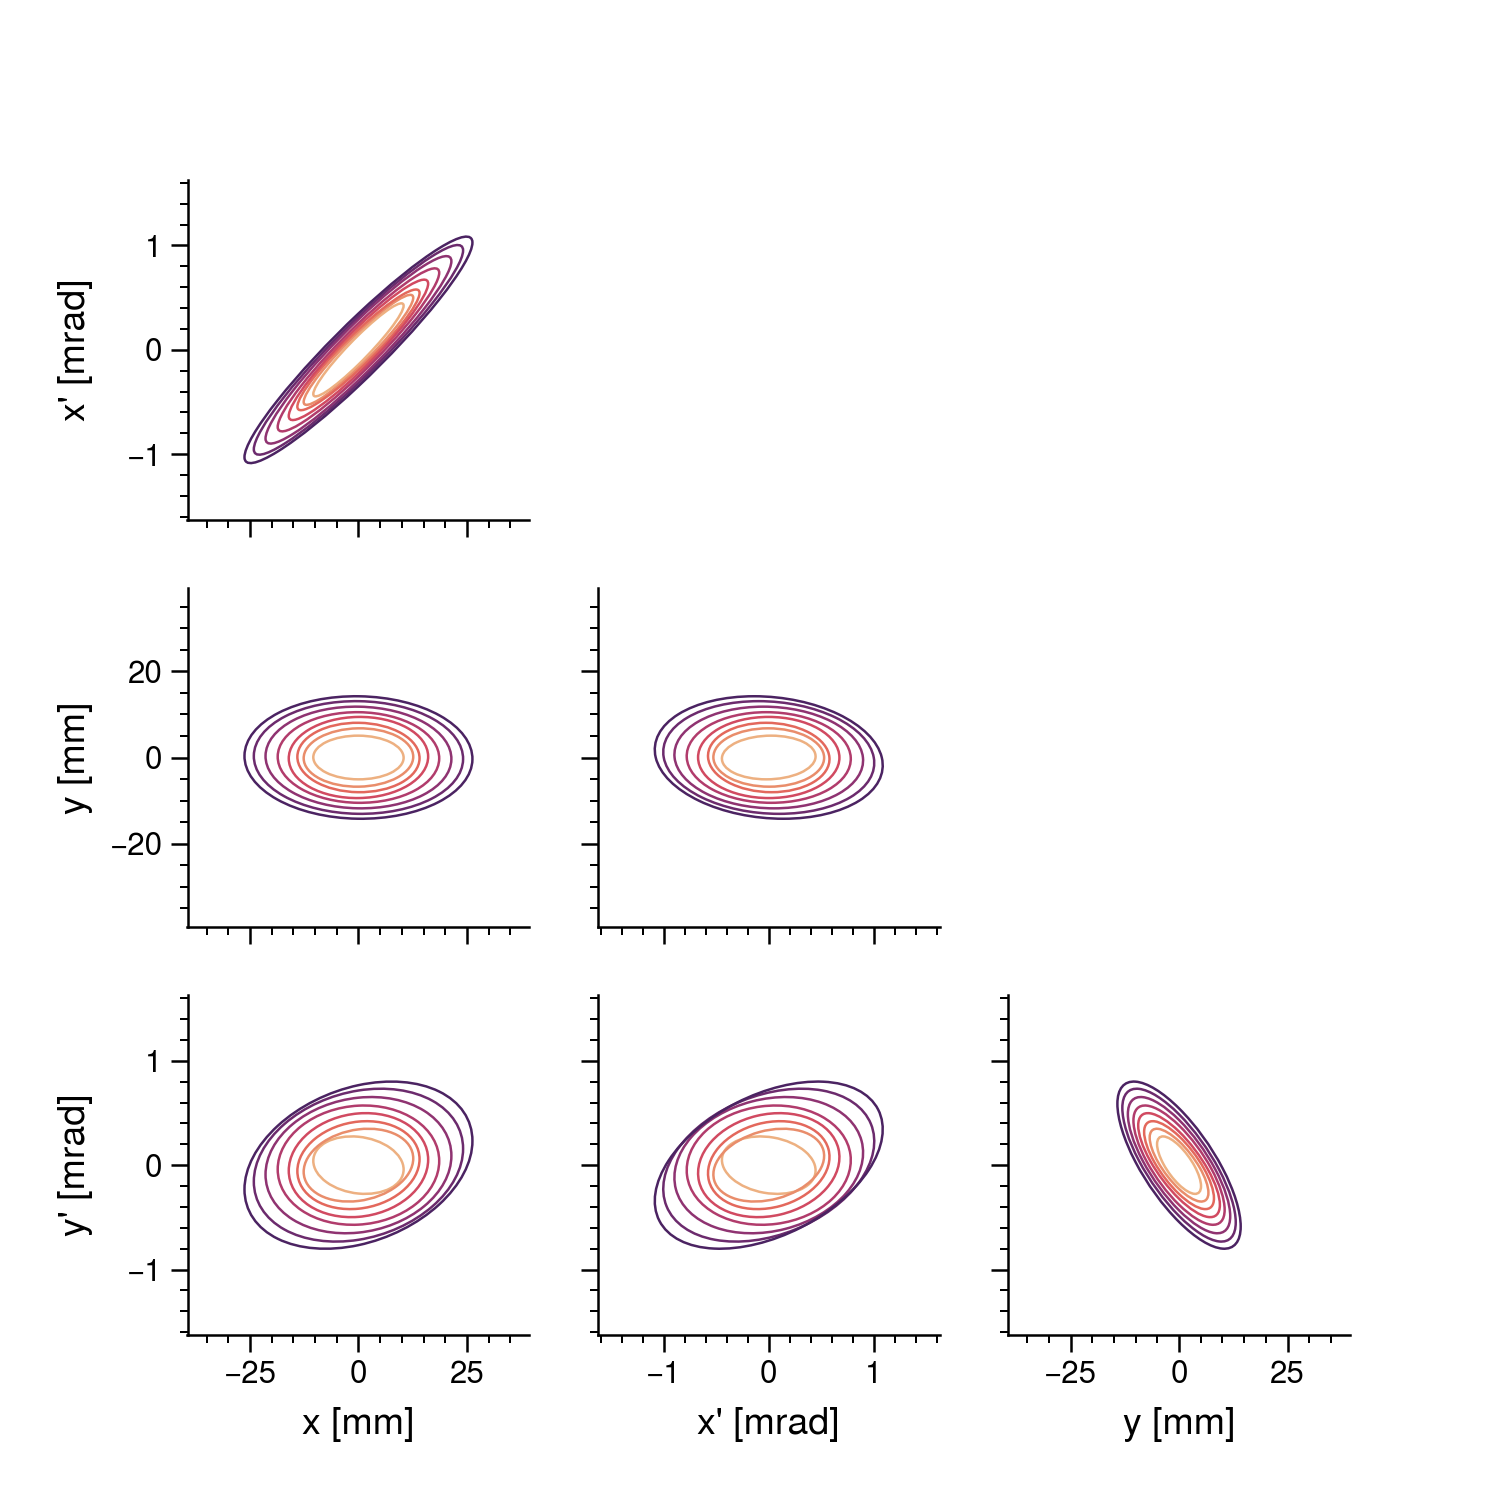
\includegraphics[width=\textwidth]{Images/chapter5/exp3/corner.png}
    \end{subfigure}
    \hfill
    \begin{subfigure}[t]{0.39\textwidth}
        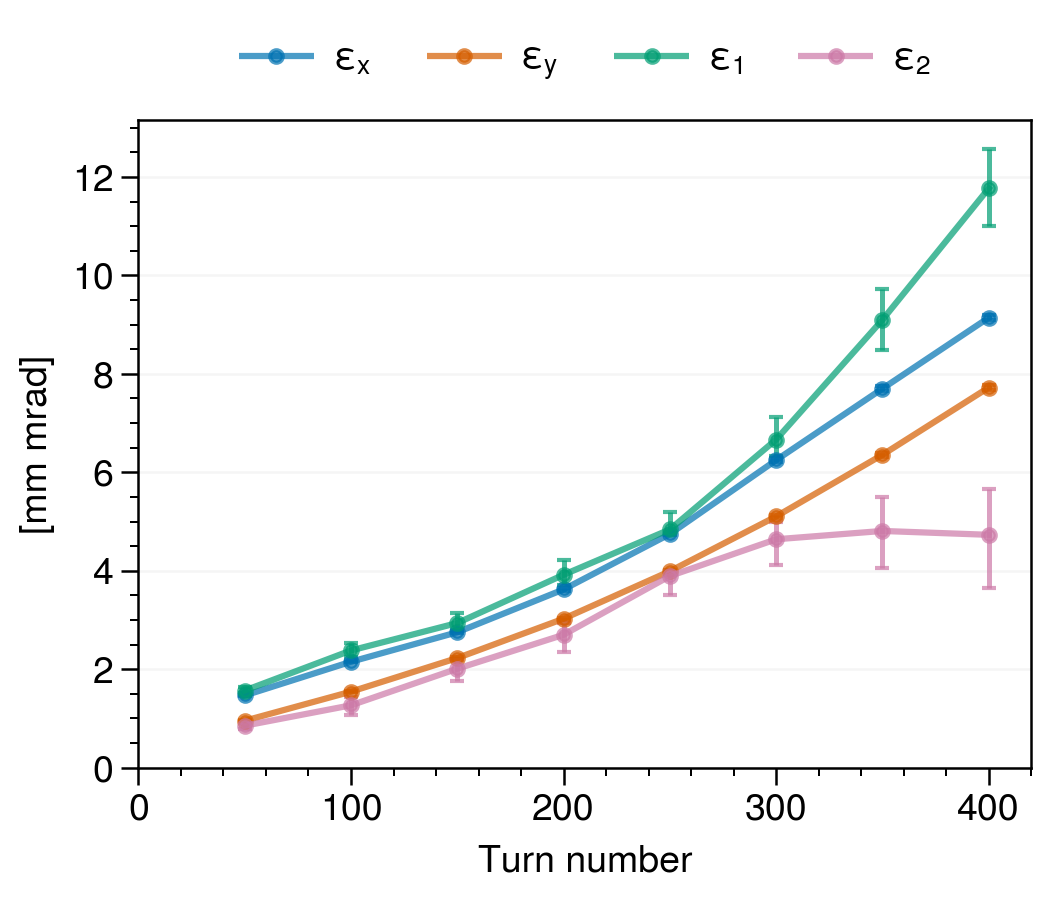
\includegraphics[width=\textwidth]{Images/chapter5/exp3/emittances.png}
    \end{subfigure}
    \caption{Reconstructed emittances and covariance ellipses from Experiment 3.}
    \label{fig:exp3_emittances}
\end{figure}
% 

Notice that $\varepsilon_{1,2}$ significantly deviate from $\varepsilon_{x,y}$ after 300 turns. This was the largest cross-plane correlation measured so far. For additional comparison with the previous experiments, it is helpful to reconstruct the covariance matrix at different locations in the RTBT, which will not change the emittances but will change the correlations between the phase space coordinates. The reconstructed cross-plane correlation coefficients are plotted in Fig.~\ref{fig:exp3_compare_corr} for Experiment 1a, Experiment 2, and Experiment 3. 
%
\begin{figure}[!p]
    \centering
    \vspace*{3.0cm}
    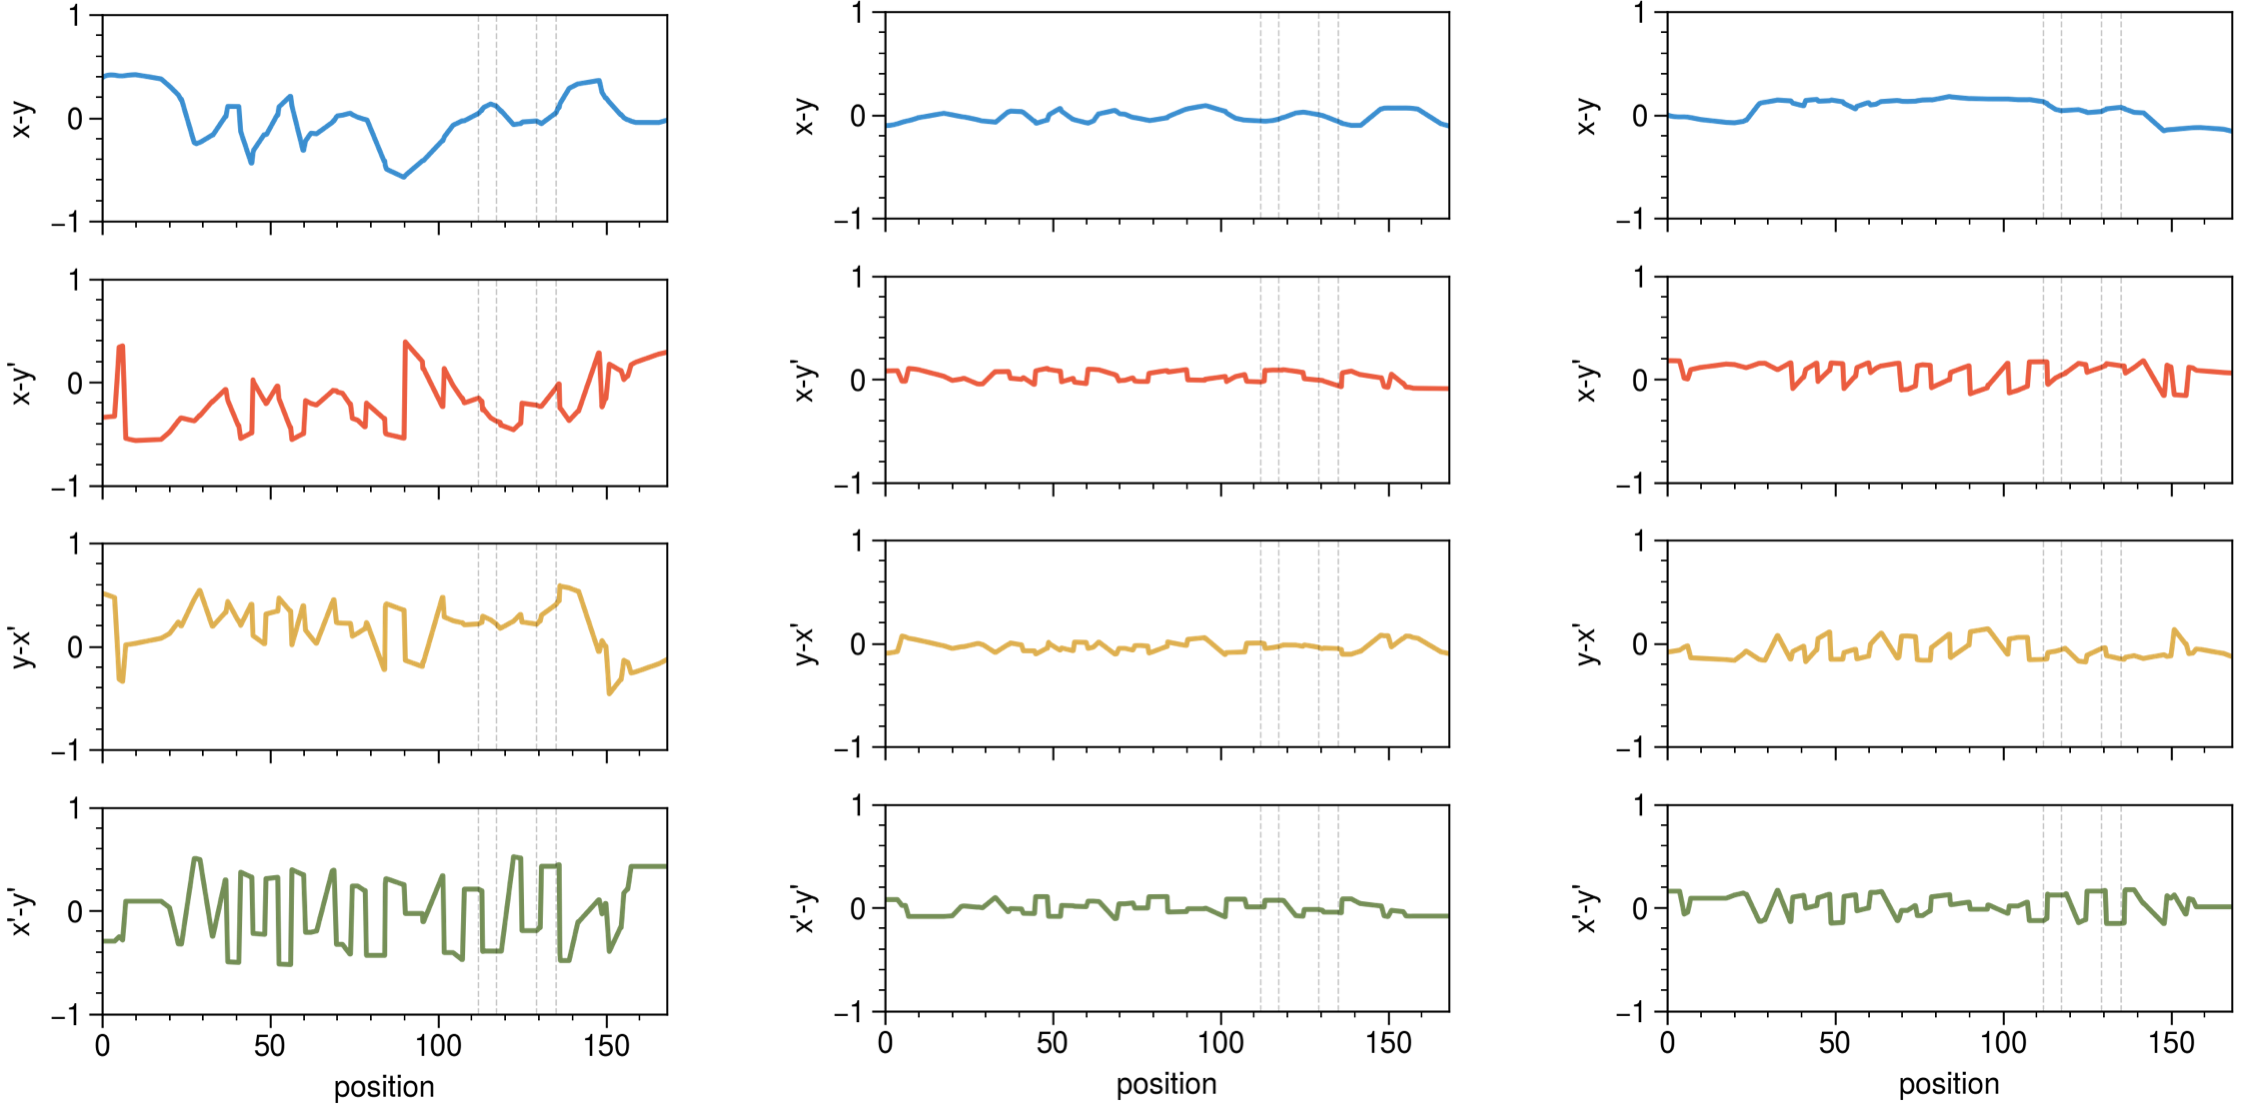
\includegraphics[width=\textwidth]{Images/chapter5/exp3/compare_corr.png}
    \caption{Reconstructed cross-plane correlation coefficients for Experiment 3 (left), Experiment 2 (middle), and Experiment 1a(right). [TO DO: ADD ERROR BARS].}
    \label{fig:exp3_compare_corr}
    \vspace*{3.0cm}
\end{figure}
%

The target scan was also performed in this experiment. The initial script calculated $15 \times 15$ phase advances, storing all the images in one array. This caused the program to crash on step 150 due to a memory error. At this point, there was not much time remaining in the control room. A second script was run that used $7 \times 7$ phase advances. Unfortunately, it was overlooked that the optics in the RTBT had already been modified for the wire-scanner measurements; eventually, the required magnet changes were too large and it was decided to stop the program. A total of 43/49 images were collected.

The pause between changing the optics, triggering the beam, and collecting the images was apparently not long enough, so there were several blanks and duplicates in the image set. The beam length was inadvertently changed from 45/64 to 15/64 of the beam length, so the distribution was not the same as in the wire-scanner measurement. A few of the images are shown in Fig.~\ref{fig:exp3_target_scan}. The $x$-$y$ correlation coefficient $r$ clearly depends on the phase advances, demonstrating that there is cross-plane correlation in the beam. But if the wire-scanner reconstruction was accurate, that beam would have displayed larger variation in $r$; it is possible that the change in beam length eliminated much of the cross-plane correlation. Another possibility is that the distribution was relatively unchanged between the two measurements, and that the wire-scanner reconstruction was inaccurate. It is difficult to draw conclusions without repeating the measurement. 

\begin{figure}[!p]
    \centering
    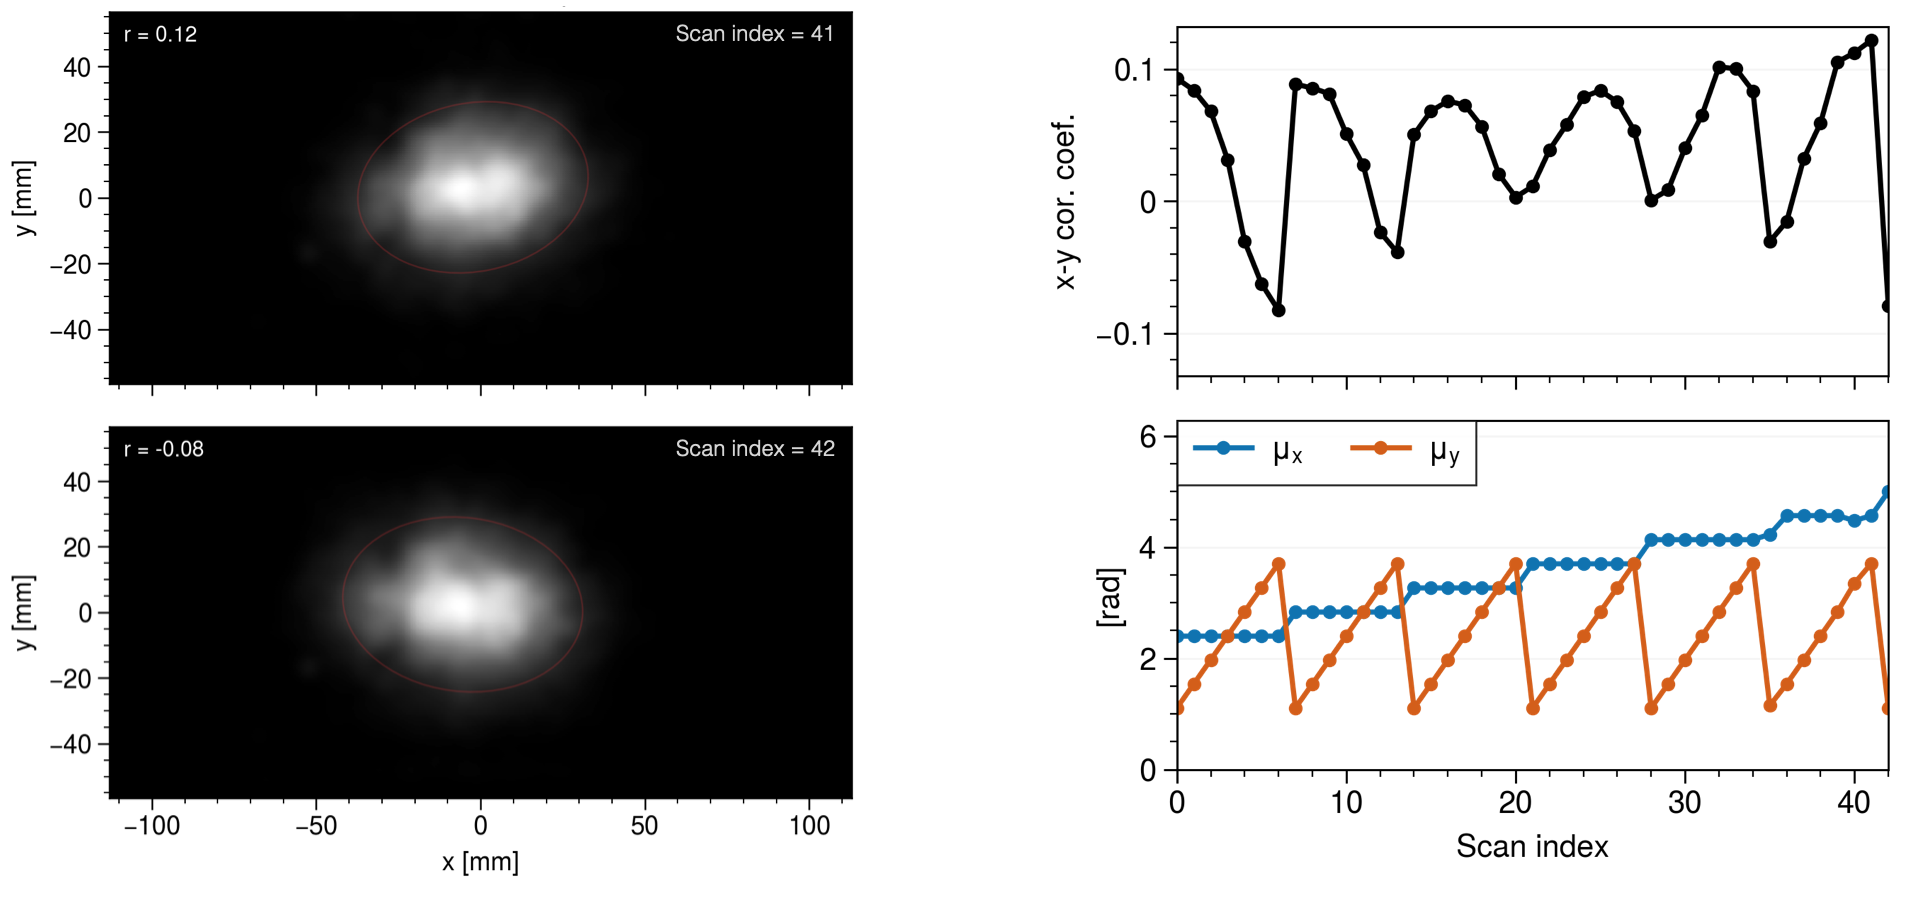
\includegraphics[width=\textwidth]{Images/chapter5/exp3/target_scan/target_scan.png}
    \caption{Scan of the phase advances at the target. Left: processed images on last two steps in the scan. Top right: $x$-$y$ correlation coefficients computed from the images. Bottom right: Phase advances at the target.}
    \label{fig:exp3_target_scan}
\end{figure}
%

Hock's method was applied to reconstruct the distribution from the images, using two iterations of SART for each 2D reconstruction. The projections of the reconstructed distribution in normalized phase space are shown in Fig.~\ref{fig:exp3_rec_corner_Hock}
%
\begin{figure}[!p]
    \centering
    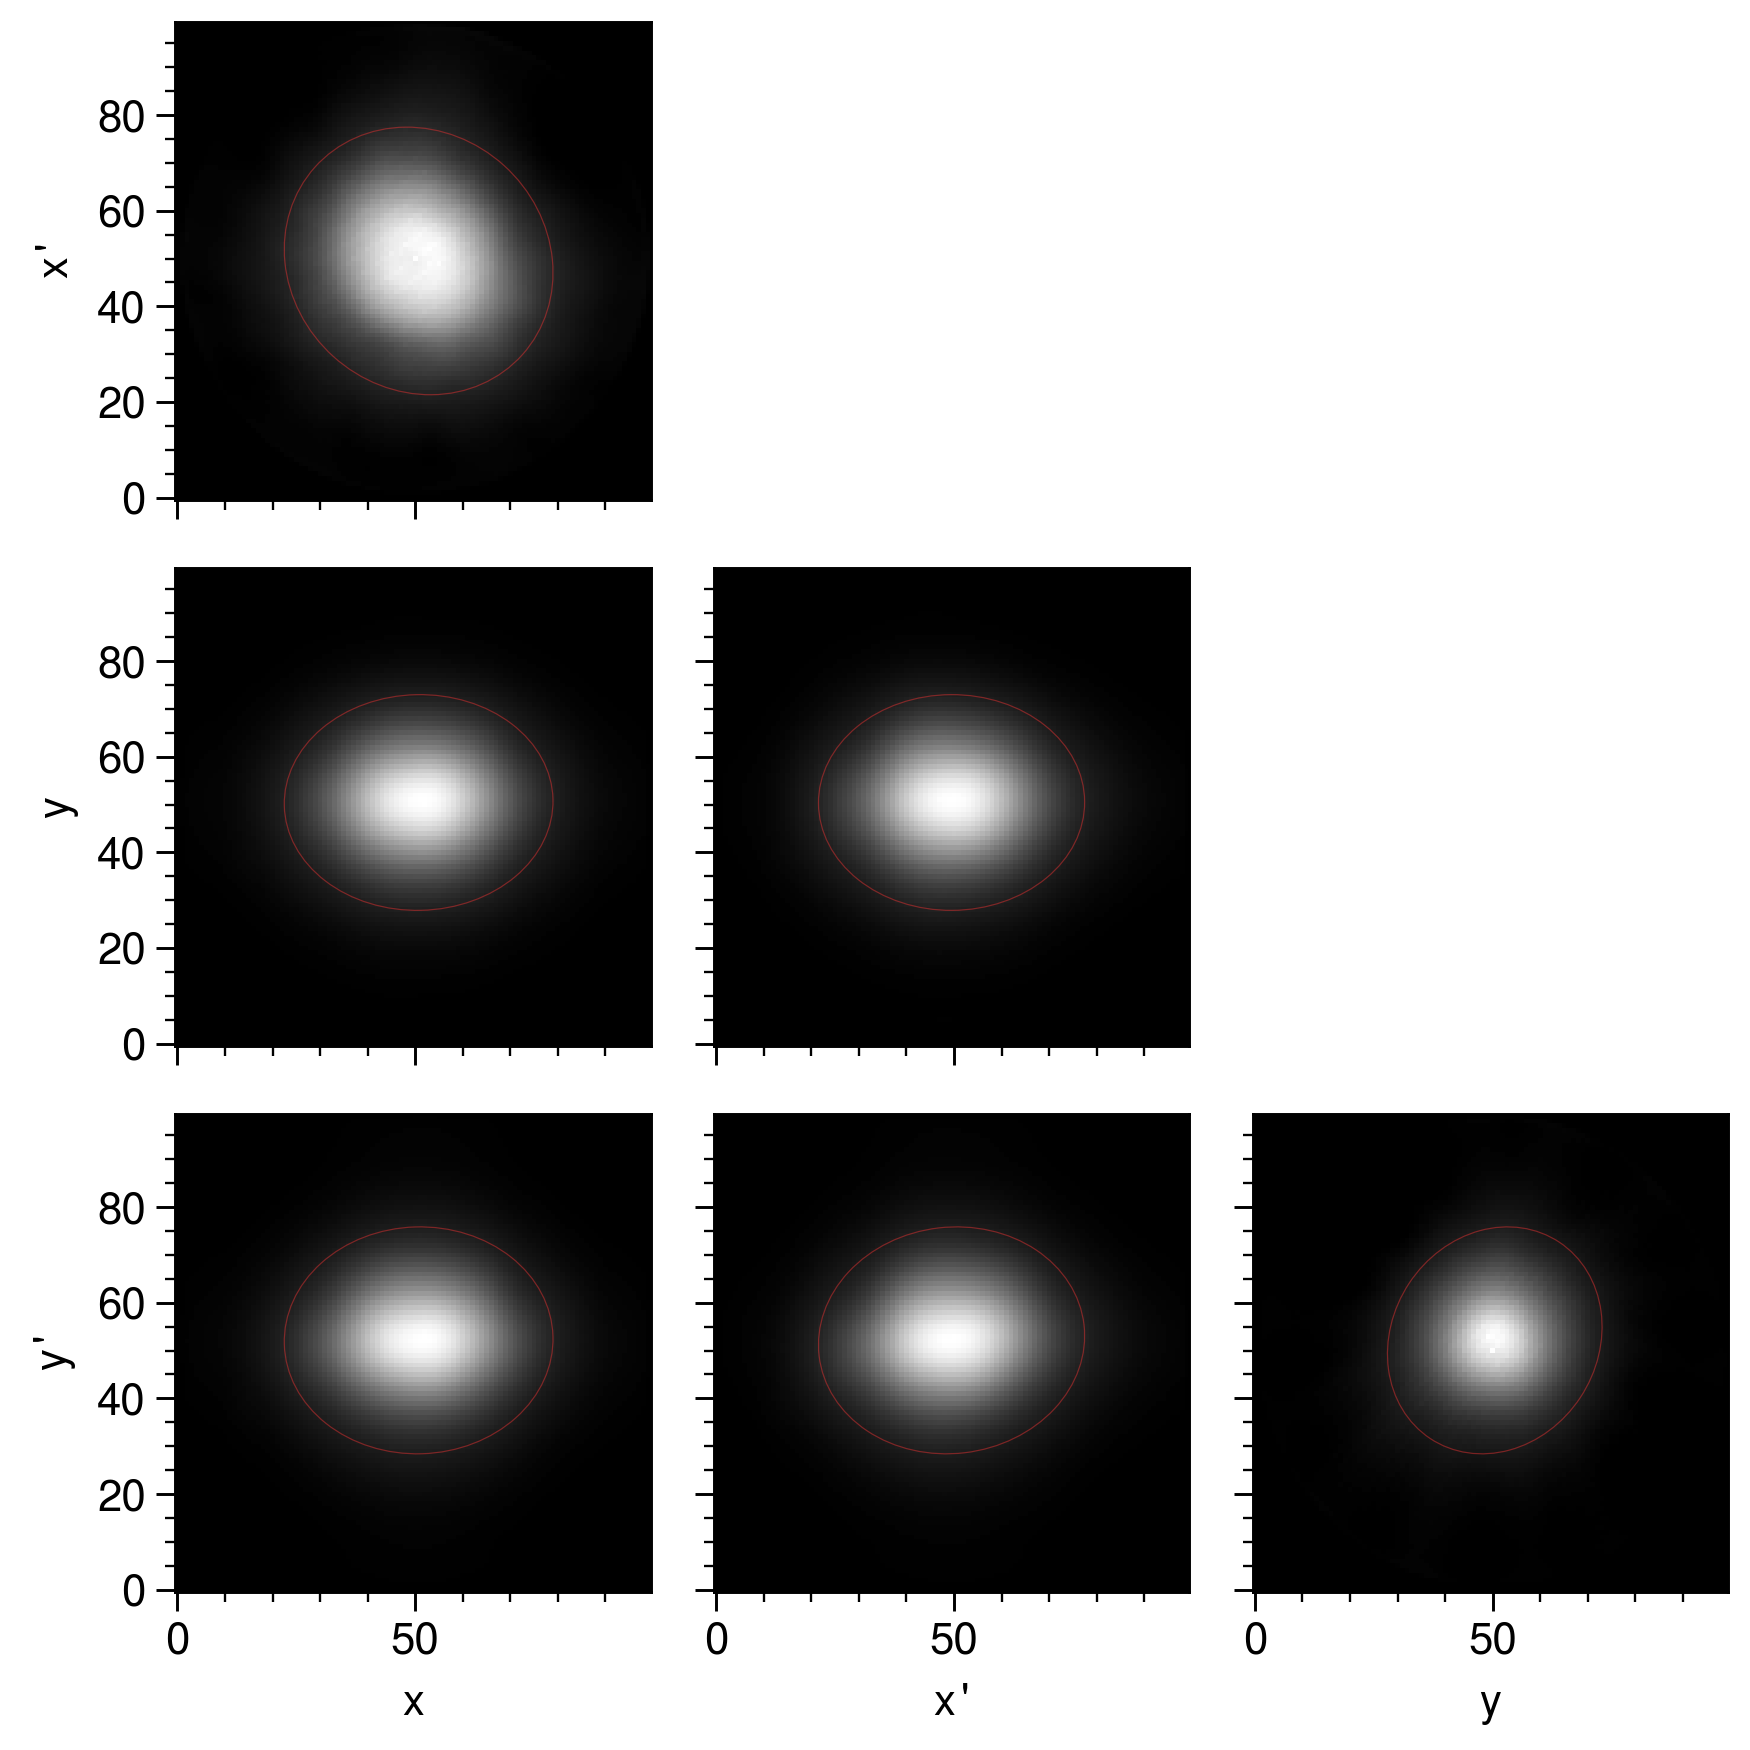
\includegraphics[width=0.75\textwidth]{Images/chapter5/exp3/target_scan/rec_corner_Hock.png}
    \caption{Projections of the reconstructed normalized phase space using Hock's method on the target images. [TO DO: GET RECONSTRUCTION GRID.]}
    \label{fig:exp3_rec_corner_Hock}
\end{figure}
%
Only seven 1D projections are used in each 2D reconstruction. Due to the limited number of projections, the reduced beam length, and the errors in the data collection script, no importance was given to this reconstruction.

We conclude with a simulation of this experiment in Fig.~\ref{fig:exp3_sim}.
% %
% \begin{figure}[!p]
%     \centering
%     \begin{subfigure}{0.85\textwidth}
%         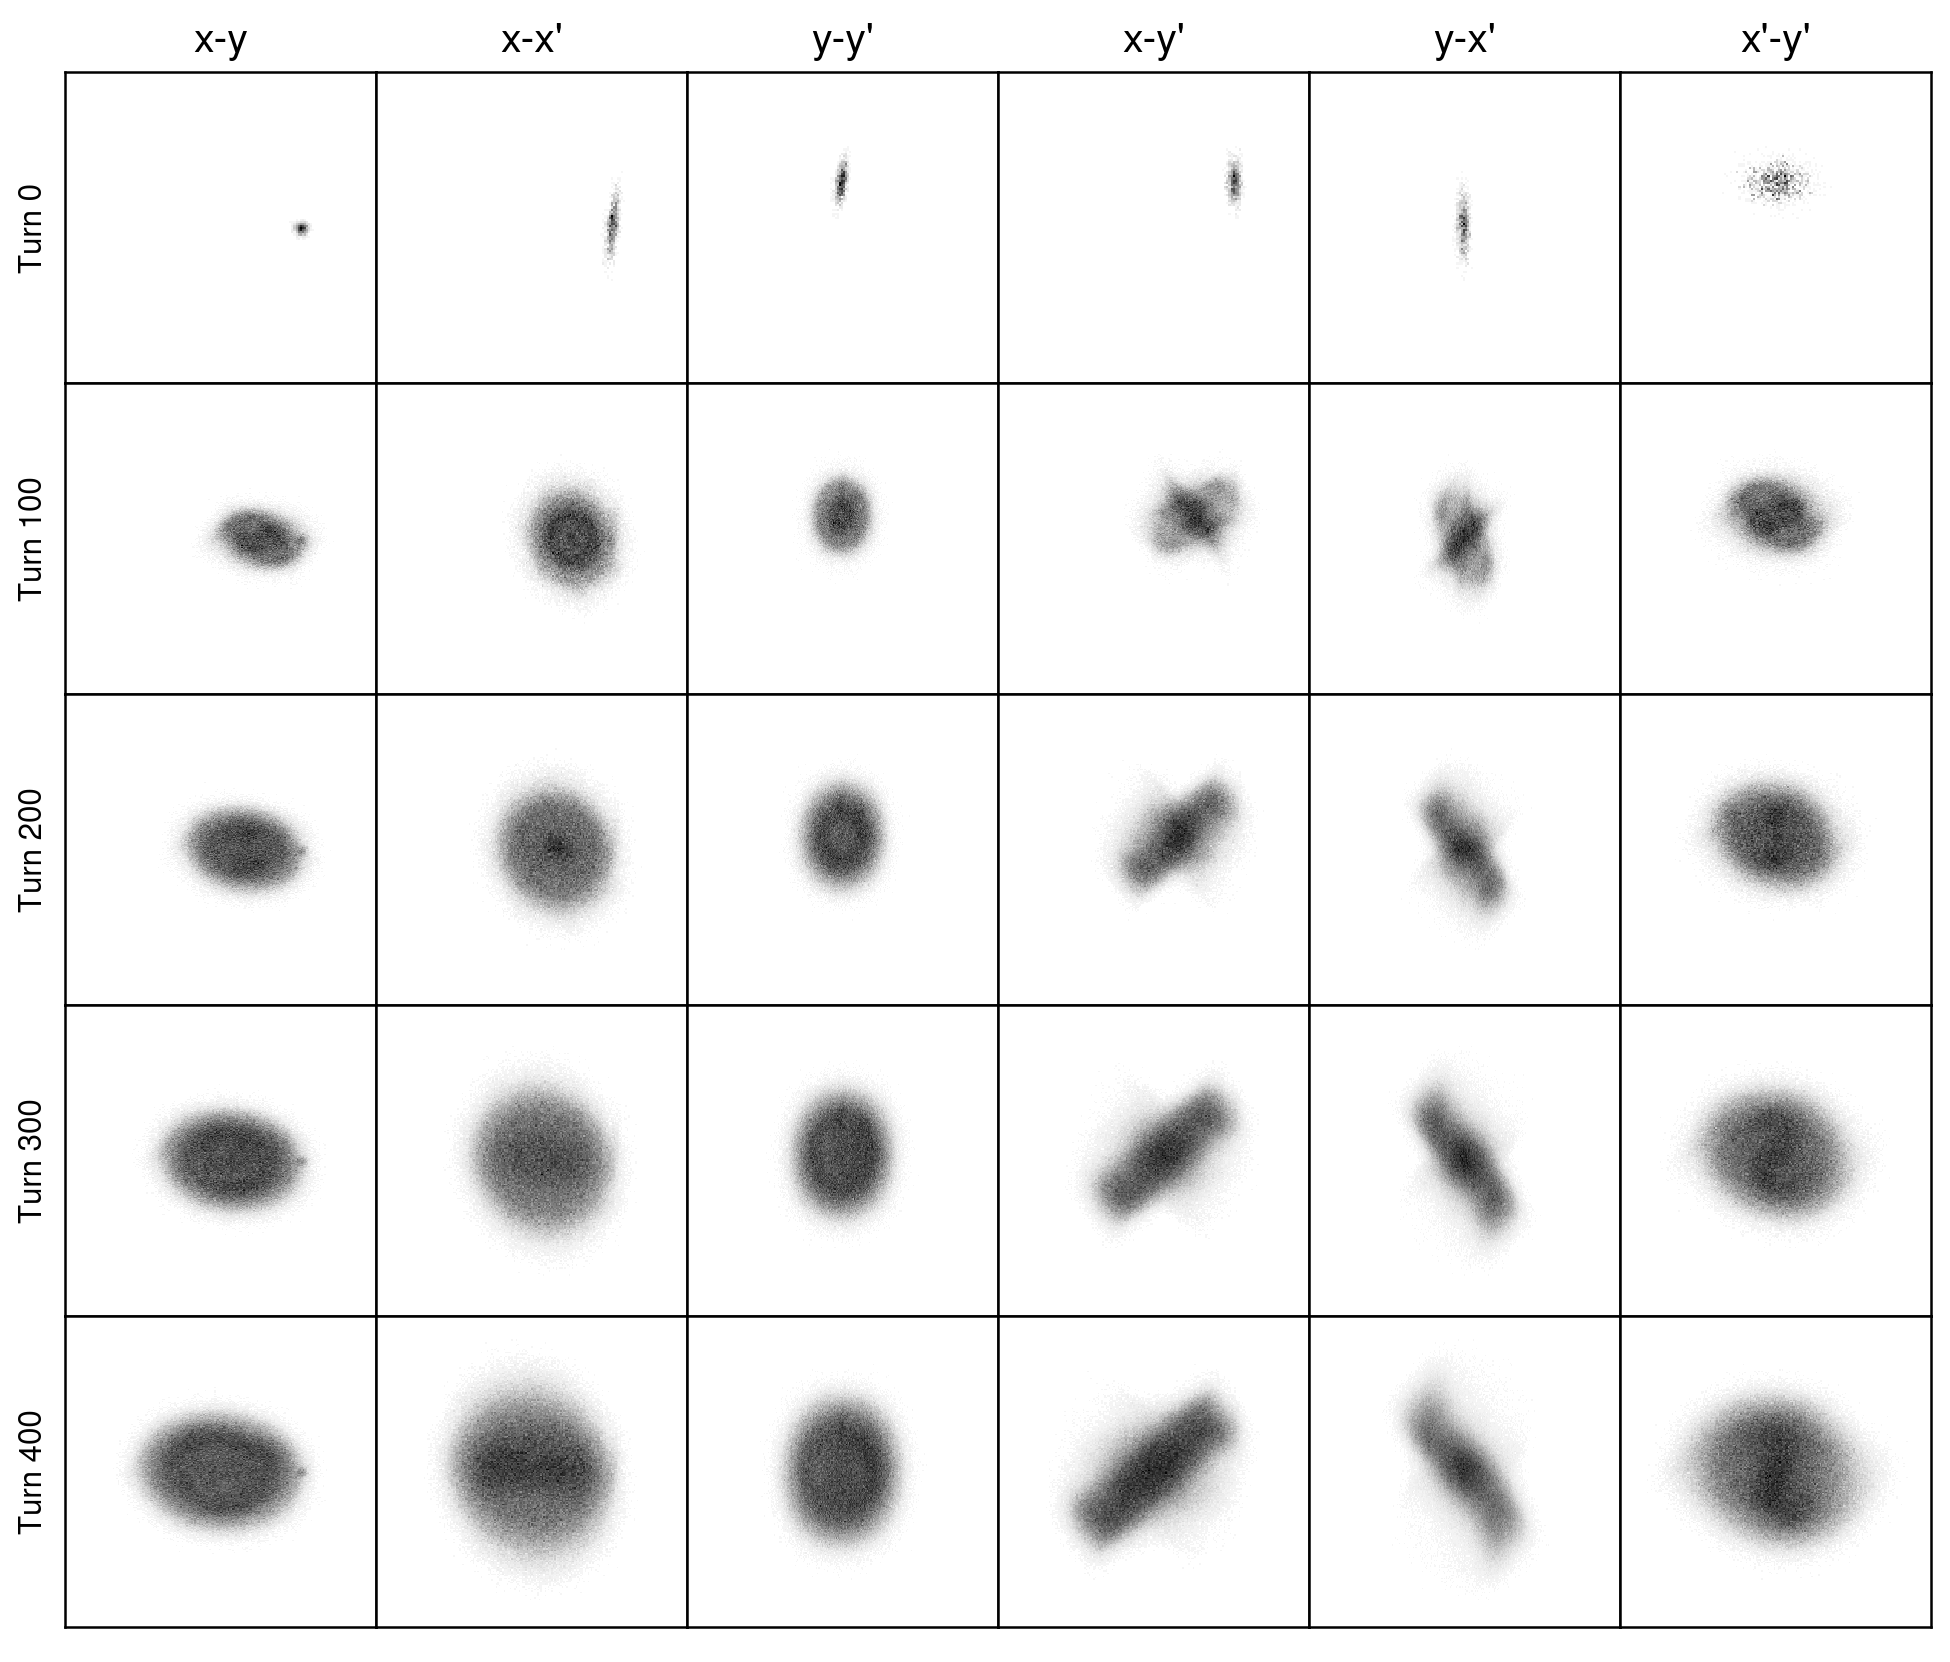
\includegraphics[width=\textwidth]{Images/chapter5/exp3/sim_snapshots.png}
%     \end{subfigure}
%     \vfill
%     \vspace*{1.0cm}
%     \vfill
%     \begin{subfigure}{0.7\textwidth}
%         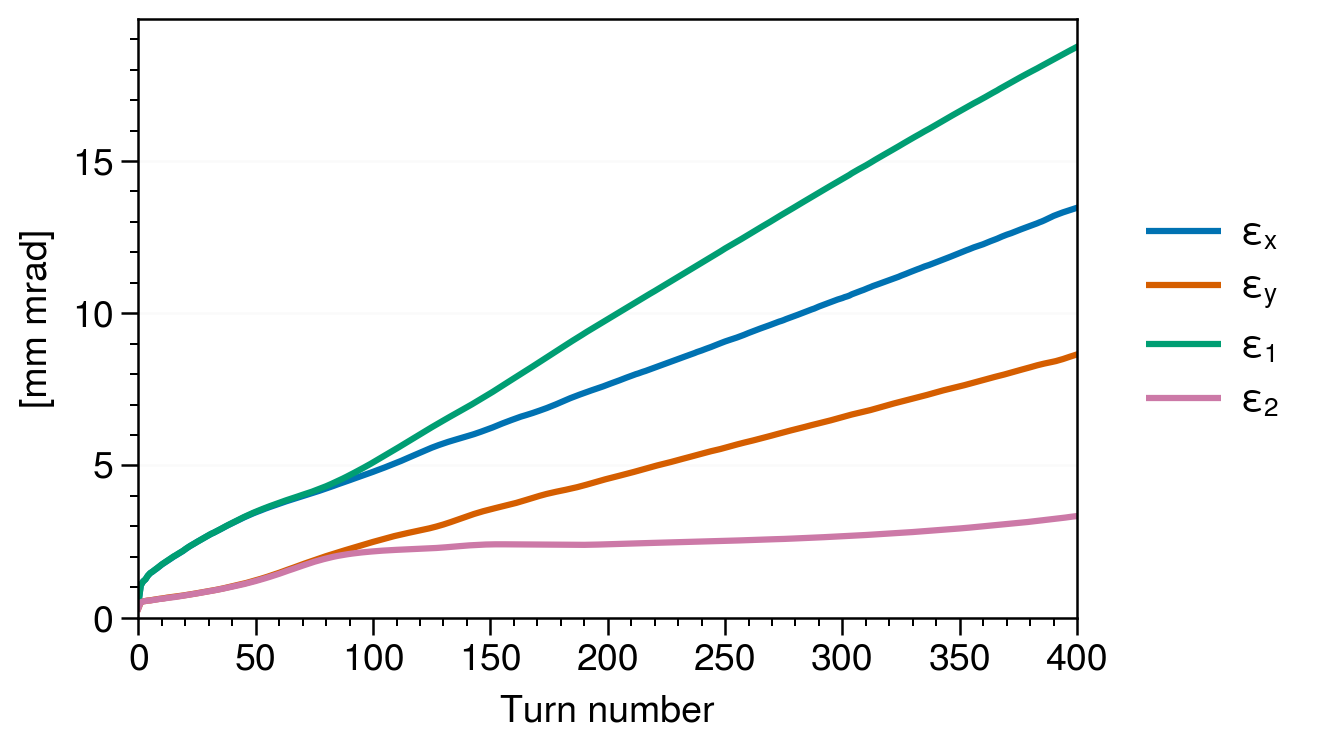
\includegraphics[width=\textwidth]{Images/chapter5/exp3/sim_emittances.png}
%     \end{subfigure}
%     \caption{Simulation of experiment 3.}
%     \label{fig:exp2_sim}
% \end{figure}
% %
This looks much closer to the best-case scenario from chapter \ref{chap-3}, even through solenoids are not present in the ring and the vertical slope from the kickers is limited. Again, the predicted ratio $\varepsilon_1 / \varepsilon_2$ is larger than what was measured; however, the simulations of Experiment 2/3 differ in a similar way to the measurements of Experiment 2/3. Namely, in Experiment 3, the smaller intrinsic emittance curve flattens as injection progresses and the final ratio $\varepsilon_1 / \varepsilon_2$ is larger than in Experiment 2. 



\section{Experiment 4}

[Jan. 2022]


\section{Summary}

The goal of the experiments in this chapter was to carry out elliptical painting in the SNS and measure the painted distribution. This has been accomplished. In Experiment 1, the Ring Injection Control (RIC) application was tested, and a procedure to efficiently measure the emittance during injection was identified. It was also found that lowering the beam energy was necessary to move the closed orbit to the foil. In Experiment 2, the beam energy was lowered to 0.8 GeV. Measurements showed that particles were injected near the closed orbit at the start of injection, and that the beam size grew with approximate square root time-dependence. A small split in the intrinsic emittances was measured near the end of injection. Simulations indicated that increasing the beam size would have a positive effect. In Experiment 3, the beam length, transverse size, and intensity were varied. The most promising case — 20\% reduction in beam intensity and 150\% increase in horizontal beam size — was investigfated in more detail. A larger split in the intrinsic emittances was measured near the end of injection. Additionally, the tilt angle of the beam image on the target was shown to depend on the phase advances at the target. In Experiment 4, [...]. These results are promising: variation of the machine parameters has a significant effect on the painted distribution.